\documentclass[main]{subfiles}

\begin{document}
    \begin{Reminder}[т. Гурса]
        \[f \in H(\Omega \setminus \{p\})\]
        \[f \in C(\Omega)\]
    \end{Reminder}

    \begin{remark} [к т. Гурса]
        Мы использовали только диф-ть $f \q \forall z \in \Omega \setminus \{p\}$\\
        Условие $f' \in C(\Omega \setminus \{p\})$ - не использовали!
    \end{remark}

    \begin{Consequence} [из т. Гурса (т. Коши для ломанной)]\
        \begin{figure}[H]
          \centering
          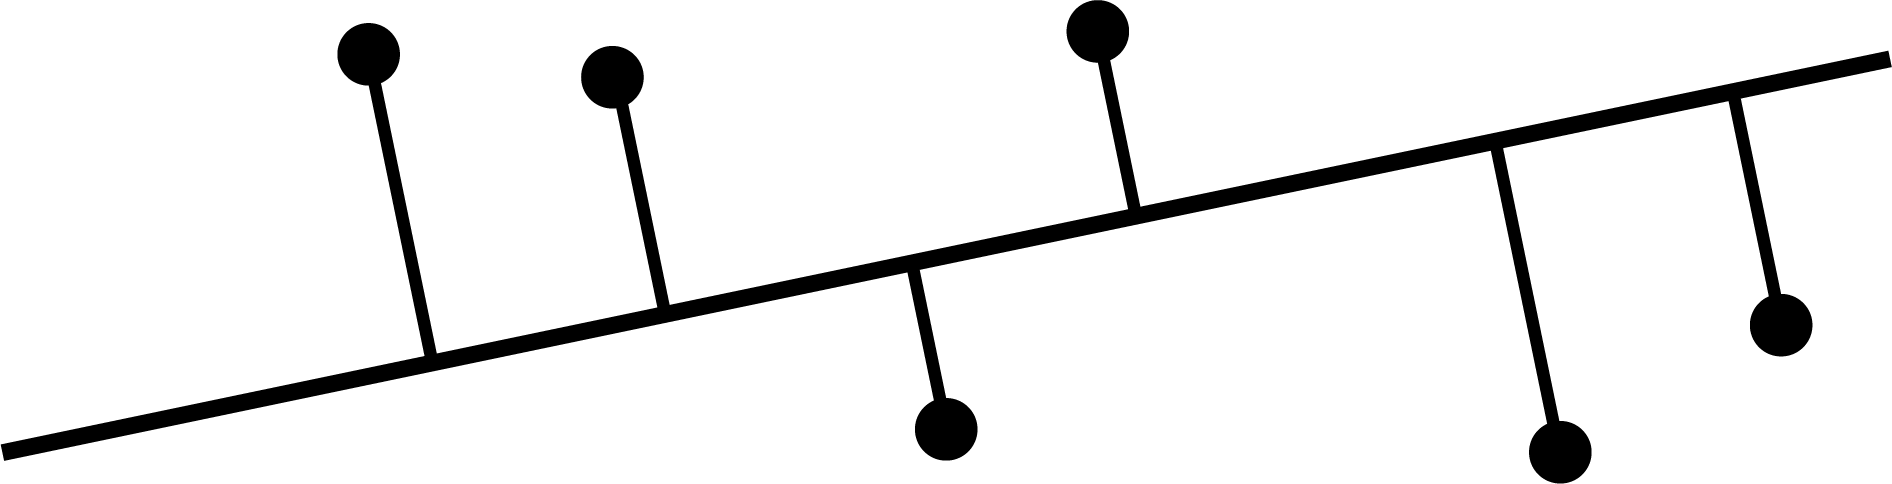
\includegraphics[width=5cm]{11_1}
        \end{figure}
        \[\int_{ABCD} = \int_{ABC} + \int_{ACD}  \]
        \[\int_{AB} + \int_{BC} + \int_{CA} \qq \int_{AC}  + \int_{CD} + \int_{DA}     \]
        \[P \text{ - замк. ломанная}\]
        \[P = \bigcup_{j = 0}^{n - 1} P_j, \q P_j - \text{ звенья}  \]
        \[P \text{ лежит в } \Omega \q \text{ вместе со своей внутр.}\]
        \[f \text{ - диф-ма } \forall z \in \Omega \setminus \{p\}\]
        \[f \in C(\Omega)\]
        \begin{figure}[H]
          \centering
          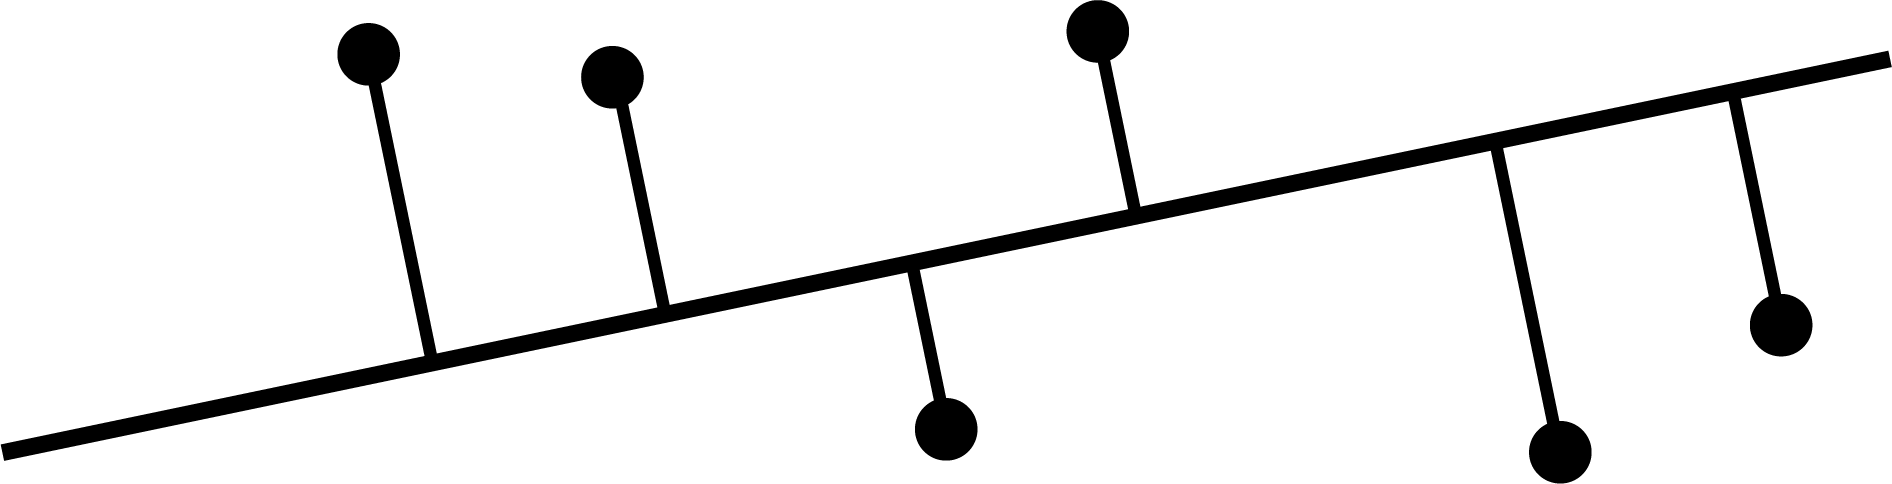
\includegraphics[width=5cm]{11_1}
        \end{figure}
        Идея доказательства - добавляем дополнительные ребра, разбиваем на треугольники,
        каждое доп. ребро встречается два раза в разных направлениях.
        \[\int_P f(z)dz = \int_P fdz + \int_{\text{доп. зв.}} fdz =
        \sum_{k} \int_{\triangle_k} f(z)dz = 0 (\text{т. Гурса})  \]
    \end{Consequence}

    \begin{Theorem}[т. Коши]
        \[L \text{ - спрям. замк. кривая, простая}\]
        \[L = \d D, \q D \subset \Omega\]
        \begin{figure}[H]
          \centering
          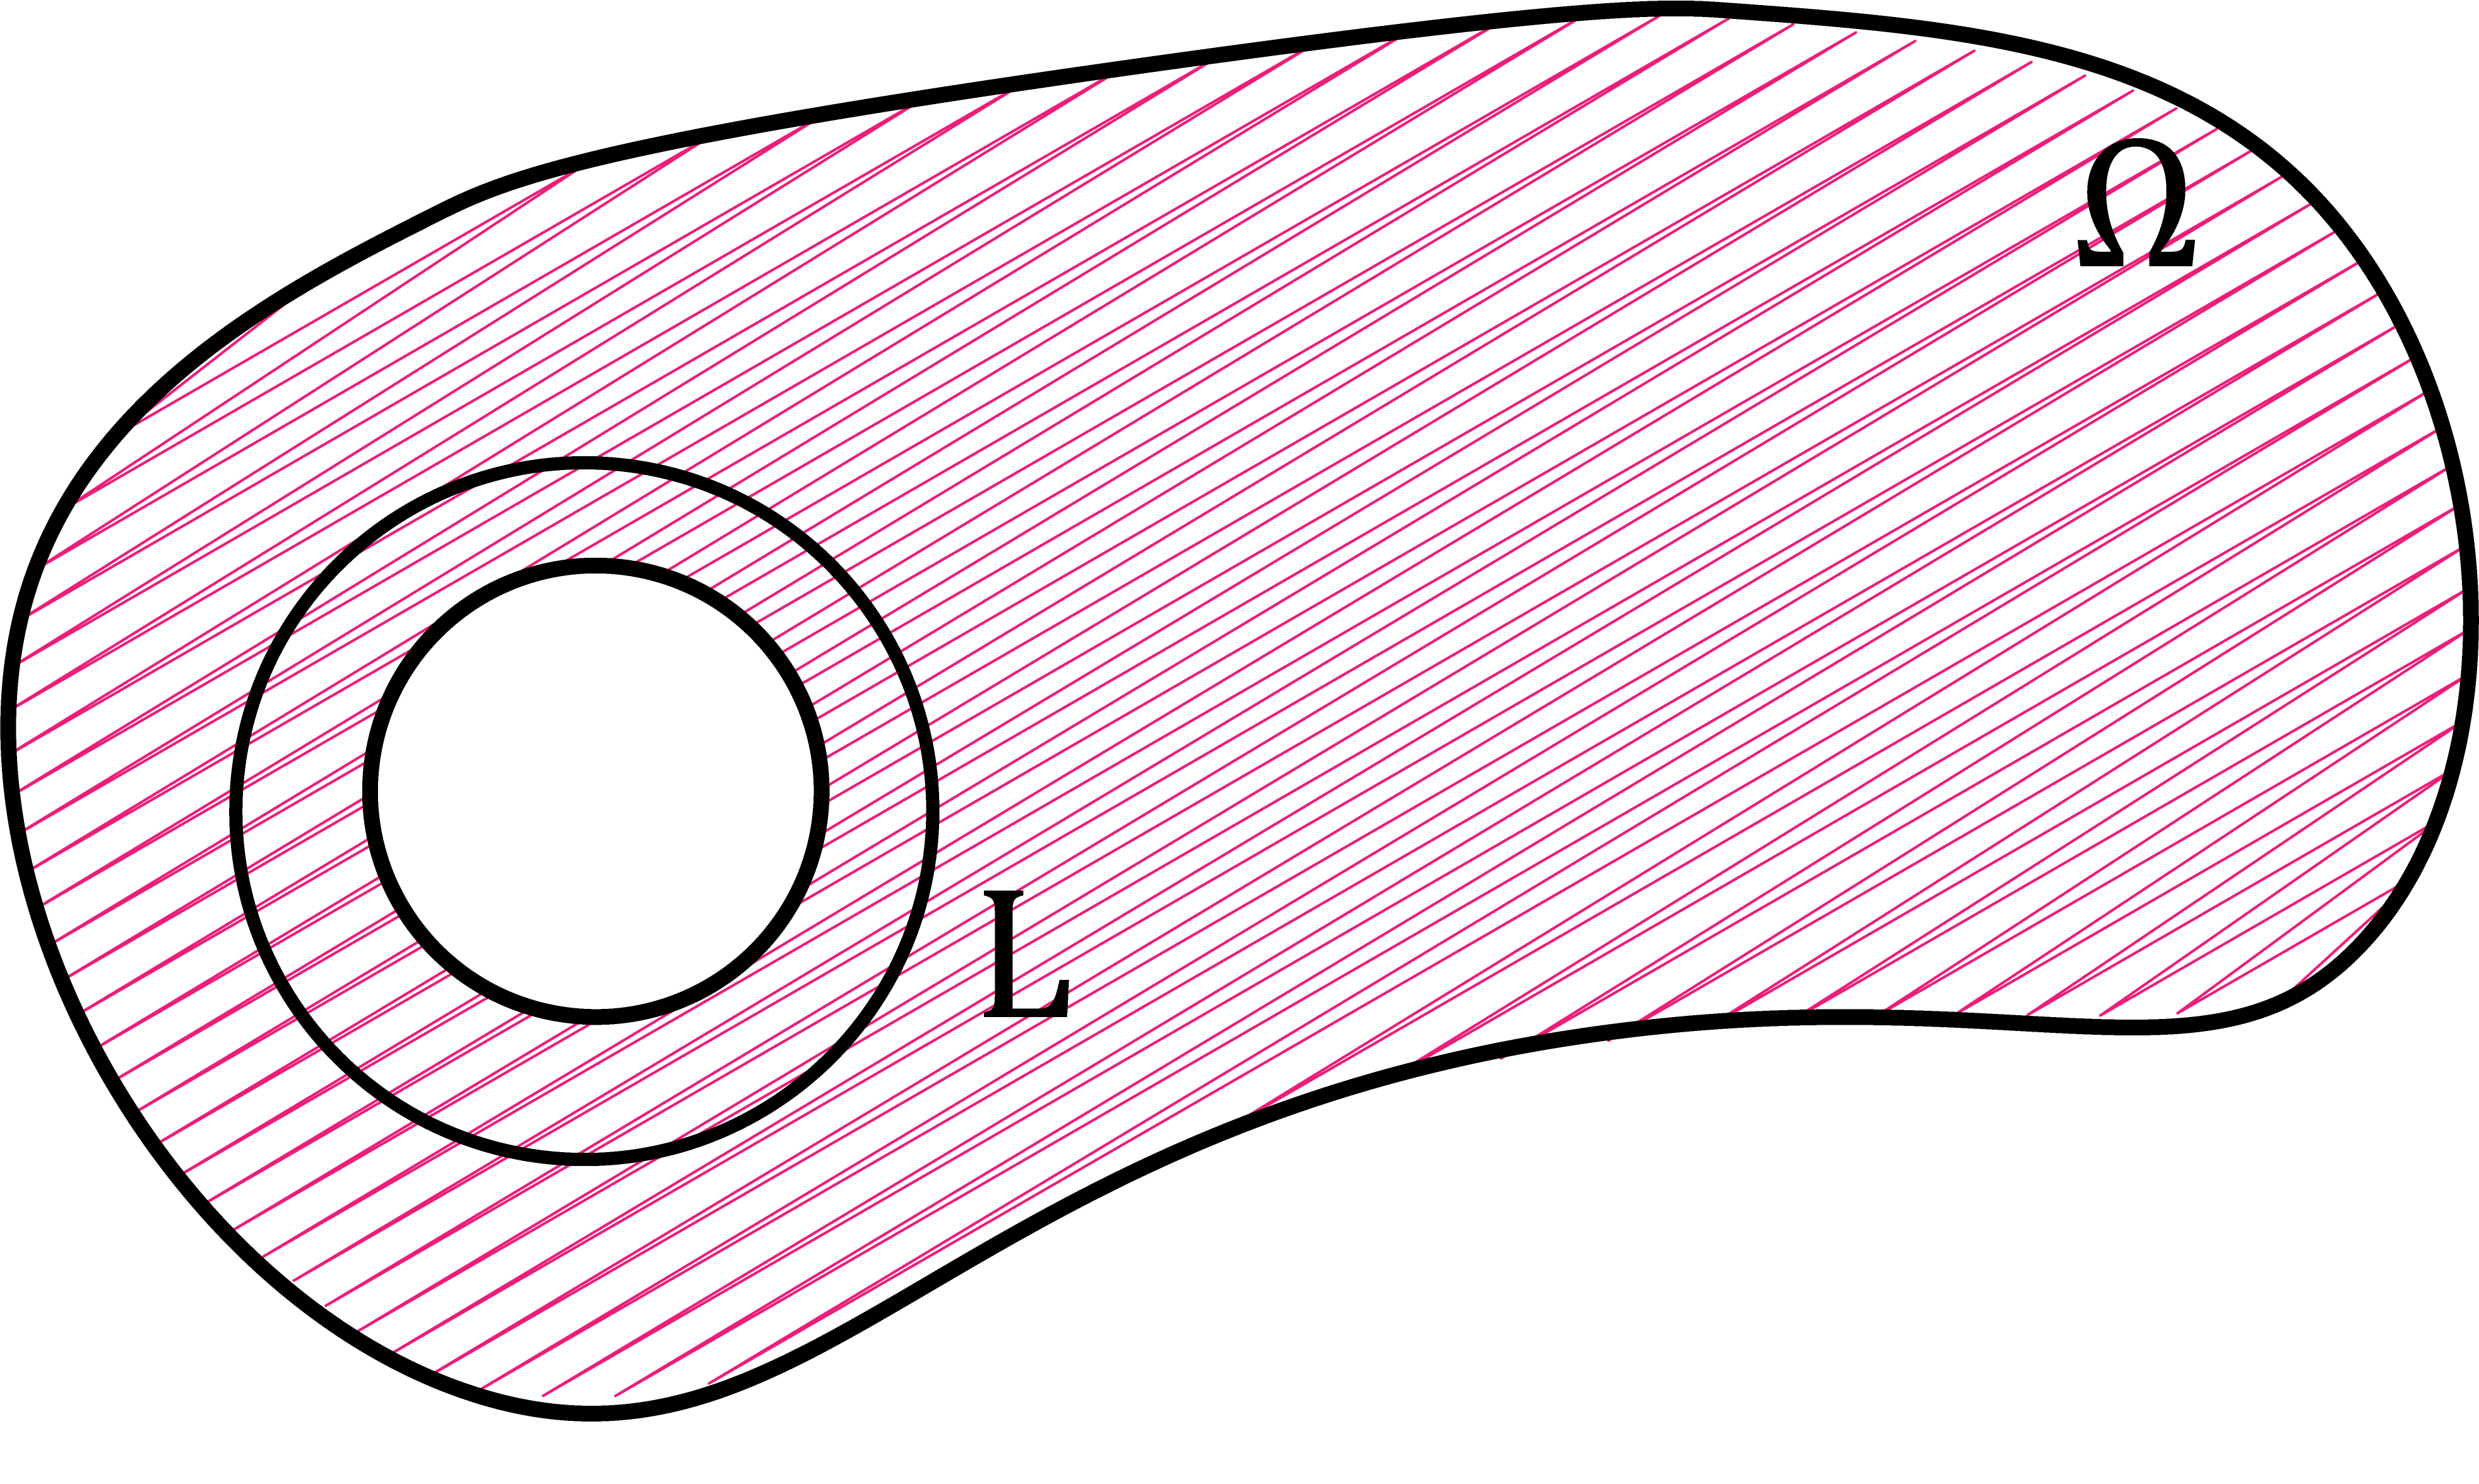
\includegraphics[width=5cm]{11_4}
        \end{figure}
        \begin{figure}[H]
          \centering
          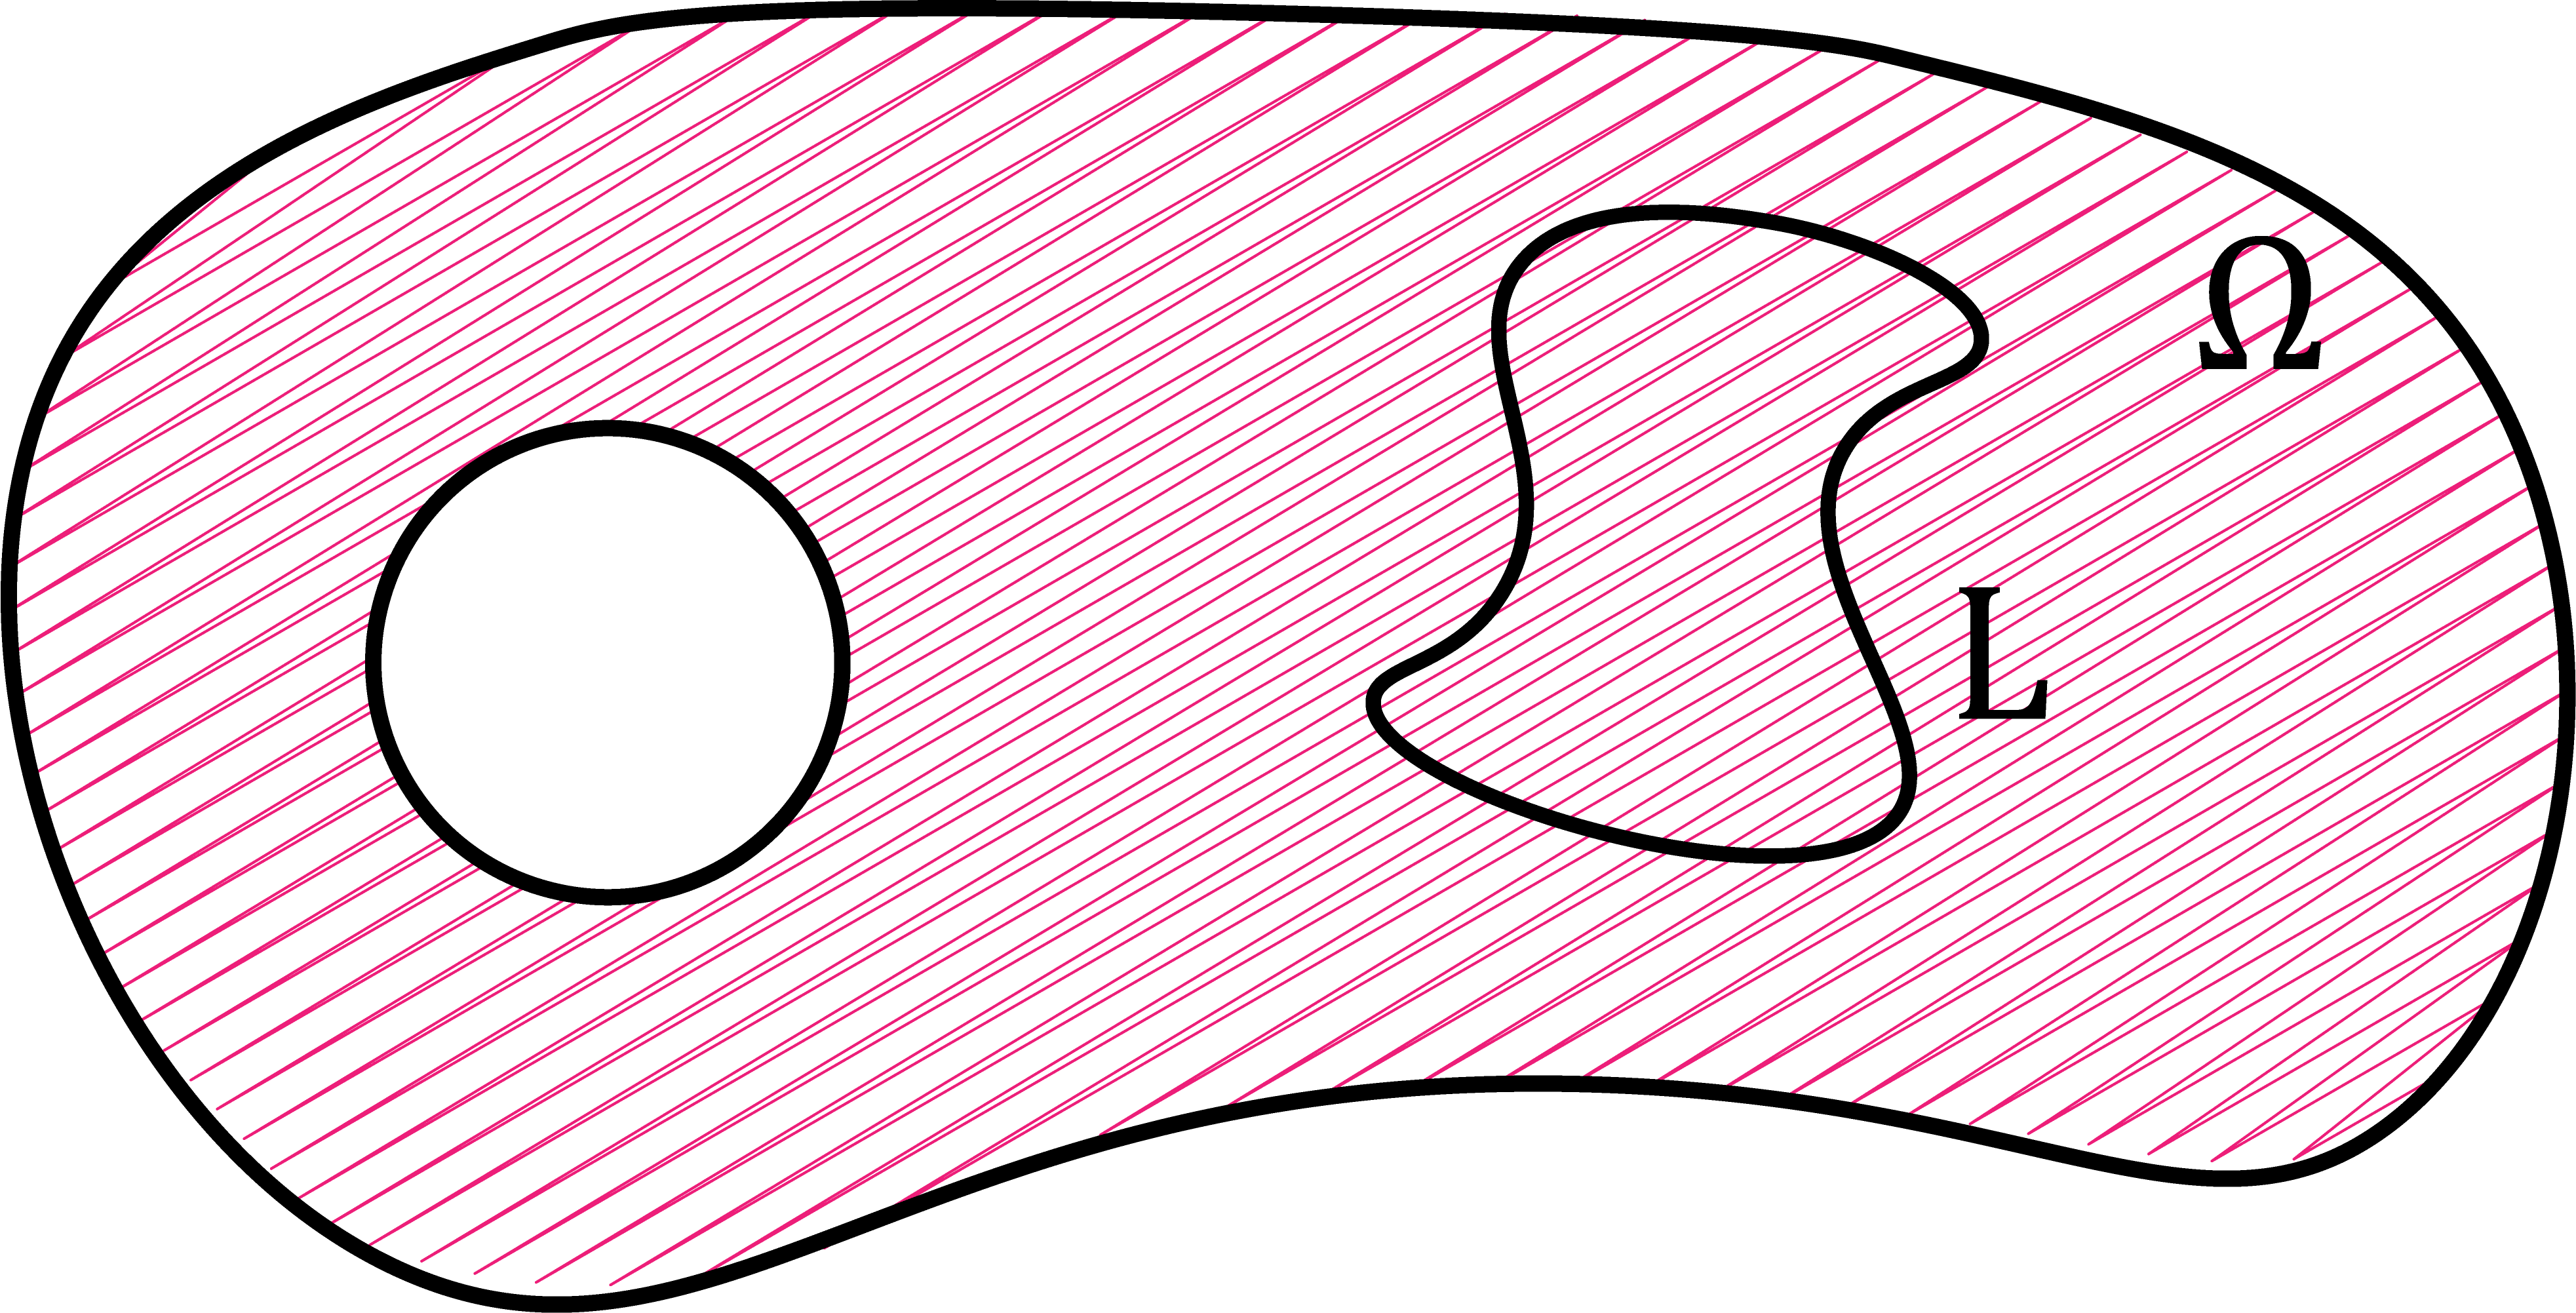
\includegraphics[width=5cm]{11_5}
        \end{figure}
        \[f \text{ - диф-ма } \forall z \in \Omega \setminus \{p\}\]
        \[f \in C(\Omega)\]
        \[\text{Тогда } \int_L f(z)dz = 0\]
    \end{Theorem}

    \begin{Example}
        \[f(z) = e^{z^2 + \cos z} \qq \int_{\gamma} e^{z^2 + \cos z} dz = 0   \]
        \[e^{z^2 + \cos z}  \in H(\CC) \text{ целая } \]
        \begin{figure}[H]
          \centering
          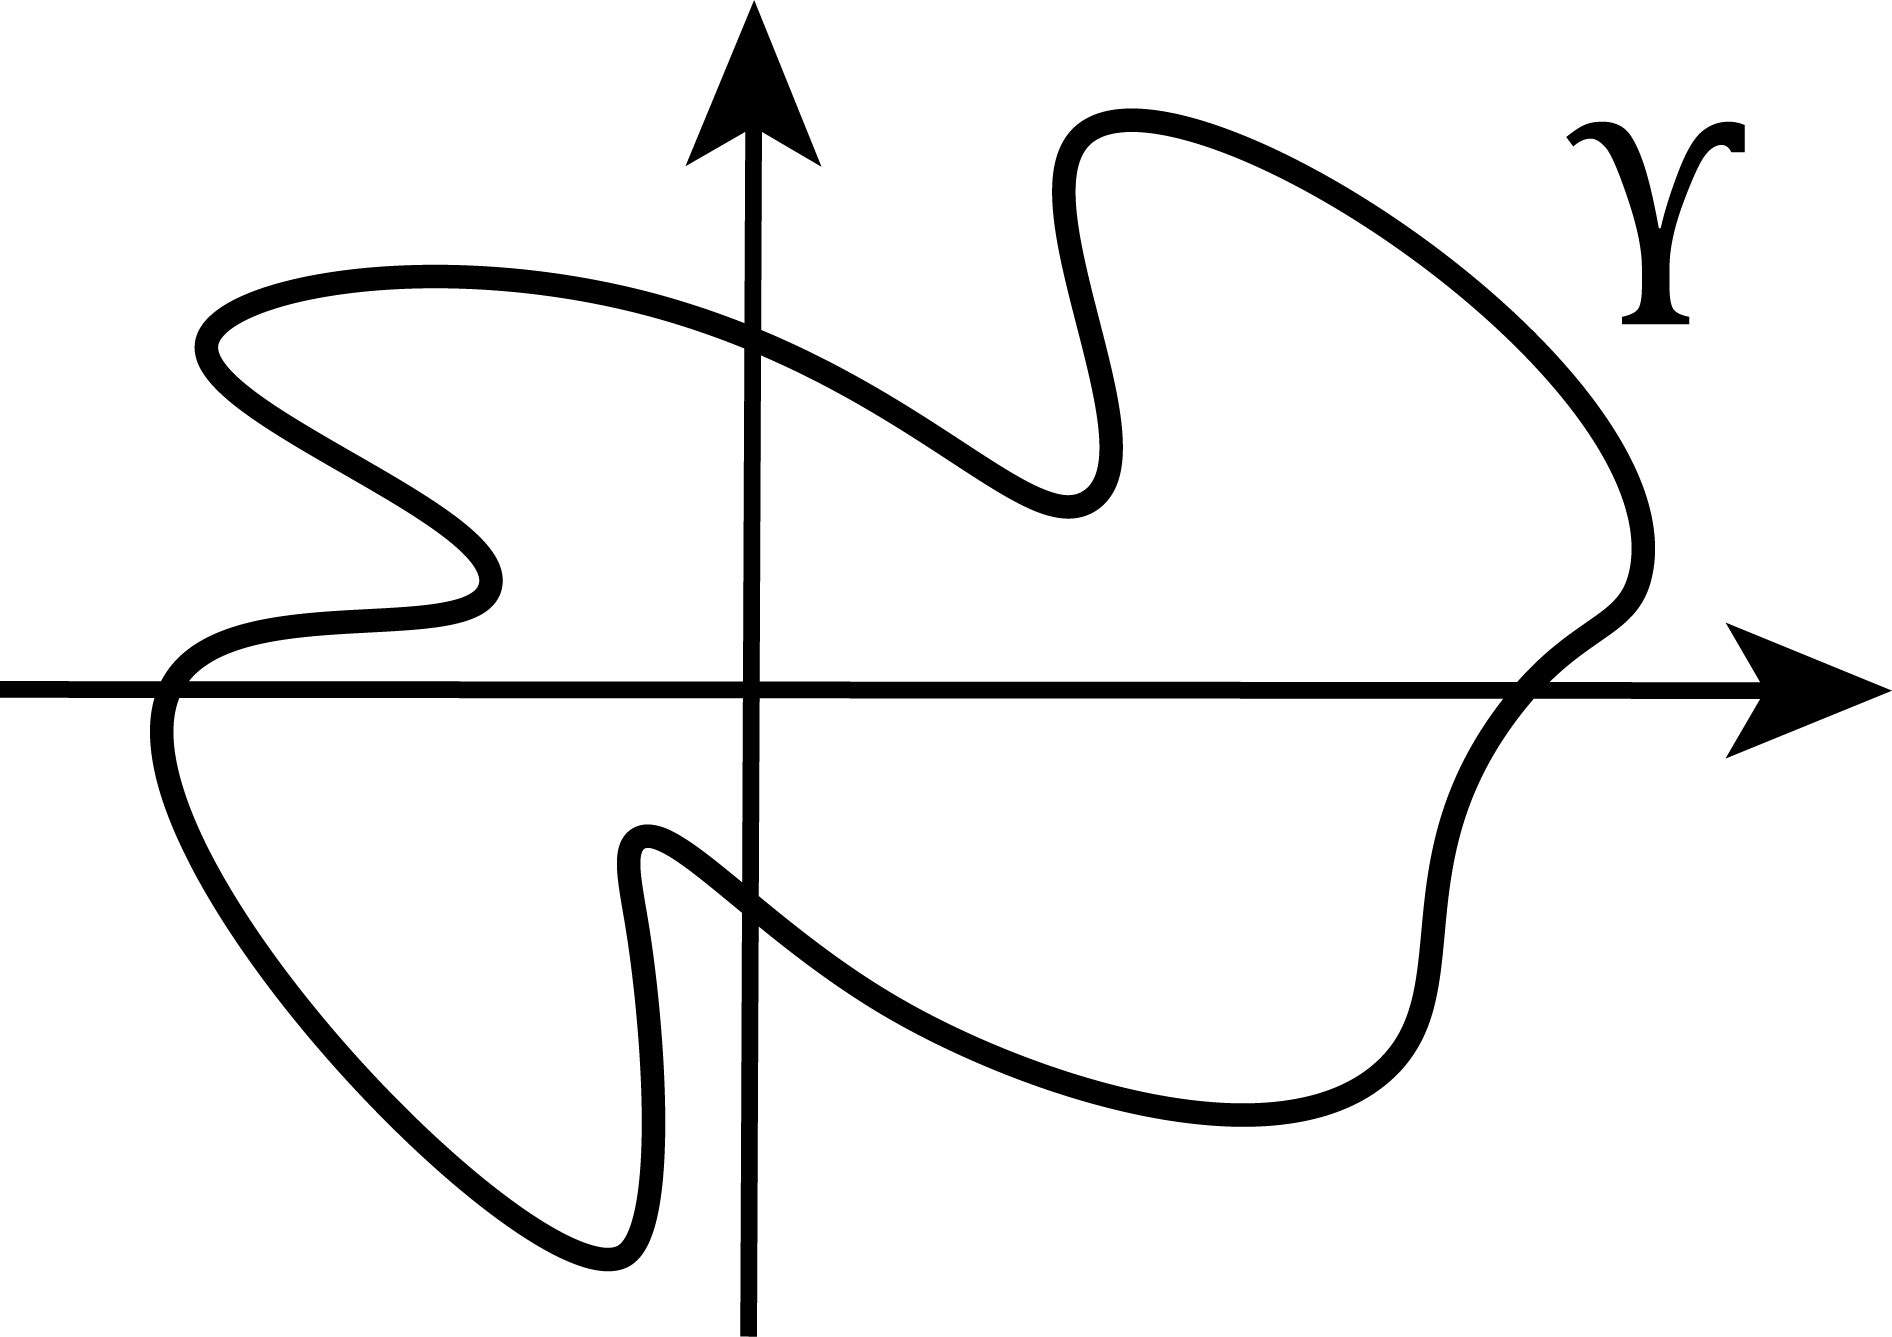
\includegraphics[width=4cm]{11_6}
        \end{figure}
    \end{Example}

    \begin{Example}
        \[\int_{\abs{z} = 1} \frac{dz}{(z - 10)(z - 20)^2} = 0\]
        Функция дифф, непр., гомом. в $\CC \setminus \{10, 20\}$
        \begin{figure}[H]
          \centering
          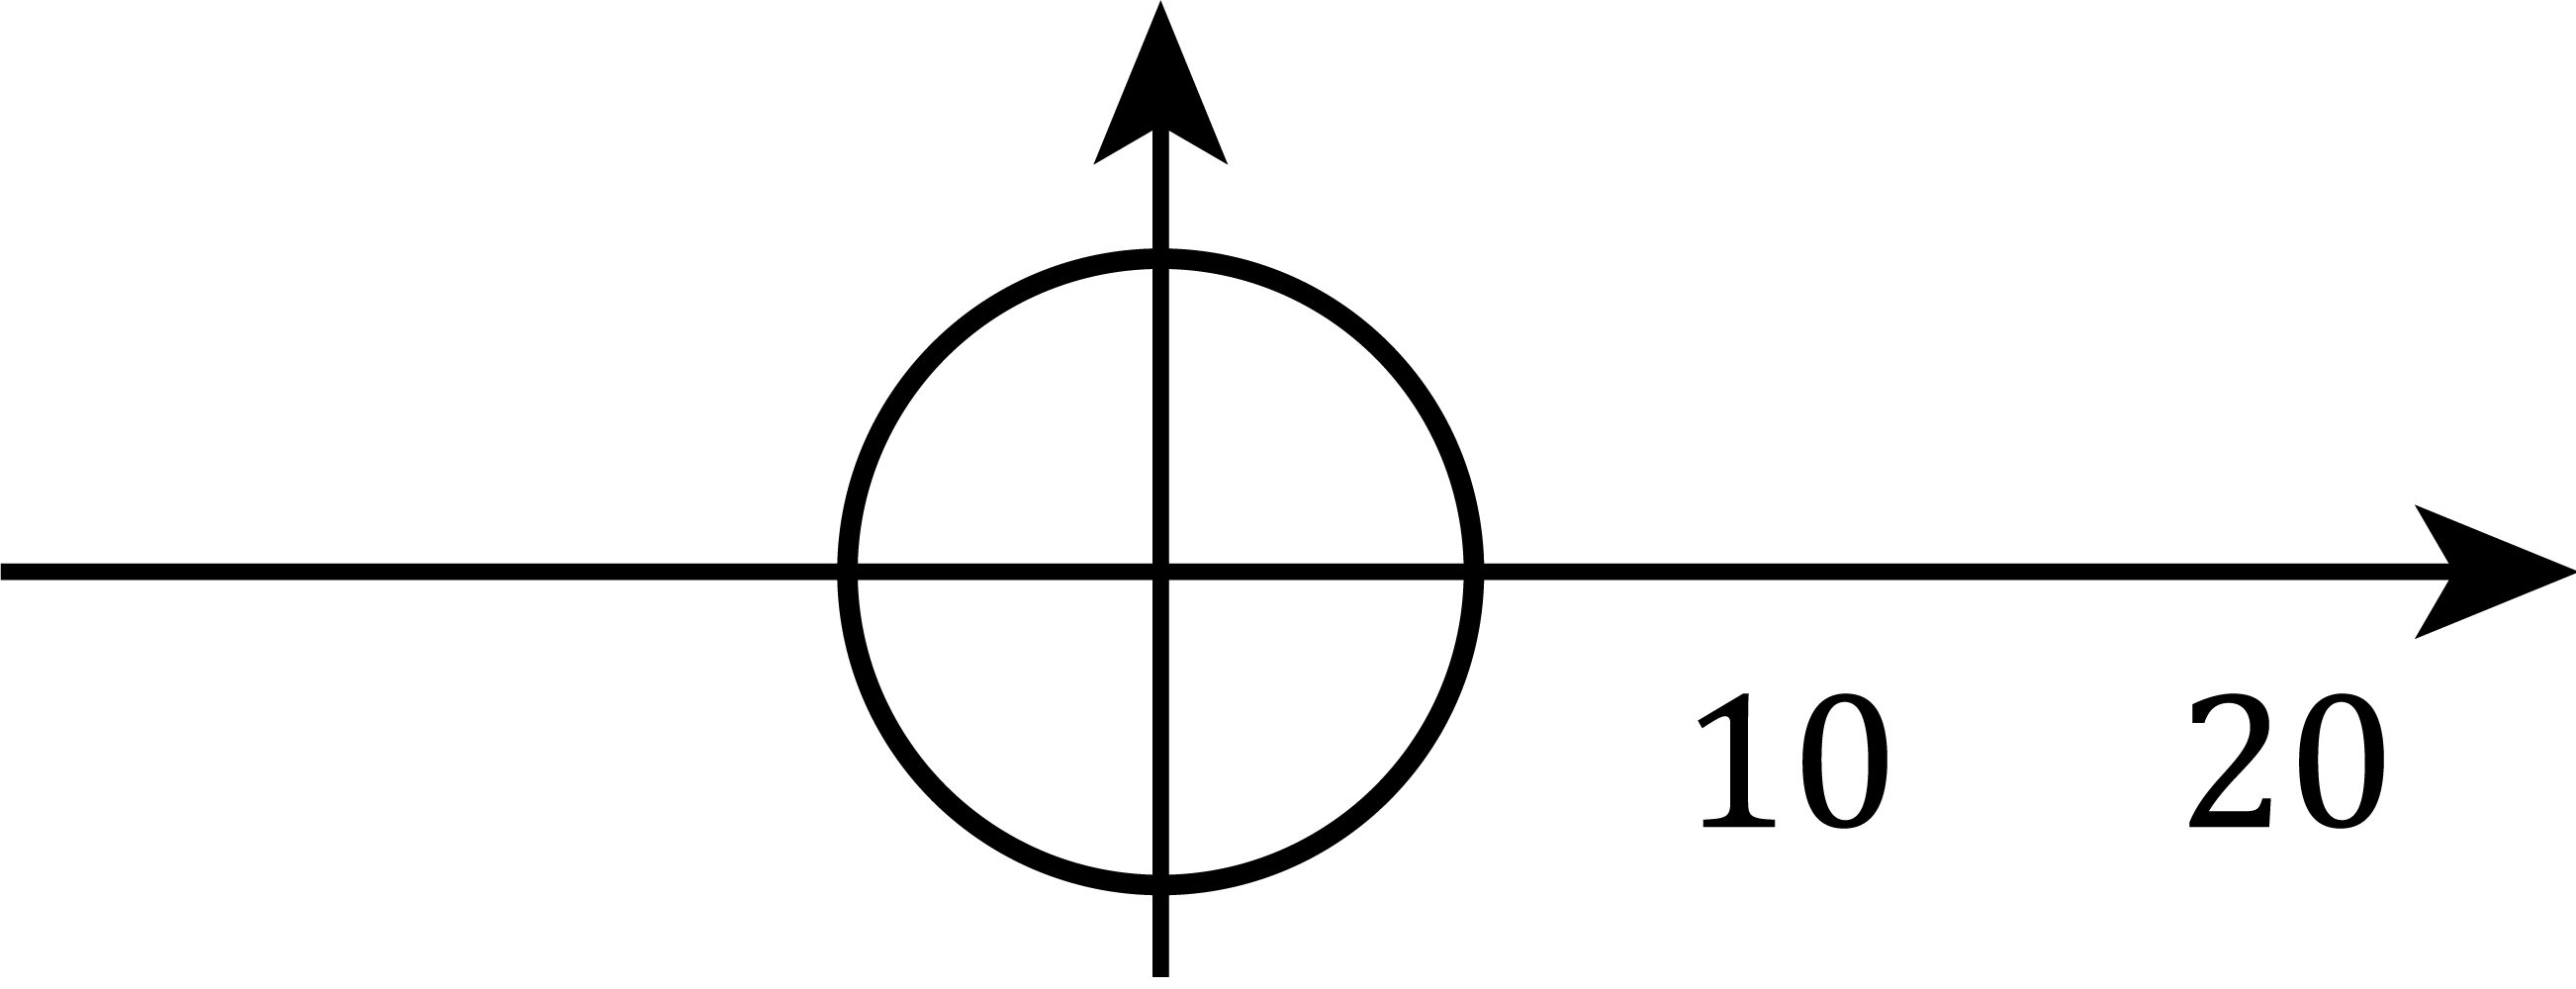
\includegraphics[width=5cm]{11_7}
        \end{figure}
    \end{Example}

    \begin{proof}
        Т.к. $f$ - непр., а $L$ - компакт., то $f$ - равномерно непр. на $L$
        \[\forall \mathcal{E} > 0 \ \exists \delta > 0 : \q \forall z_1, z_2 \q
            \abs{z_1 - z_2}
        < \delta \Ra \abs{f(z_1) - f(z_2)} < \mathcal{E}\]
        \[\widetilde{\delta} = \min(\delta,\ \frac{1}{2} \text{dist}(L, \d \Omega))\]
        \begin{figure}[H]
          \centering
          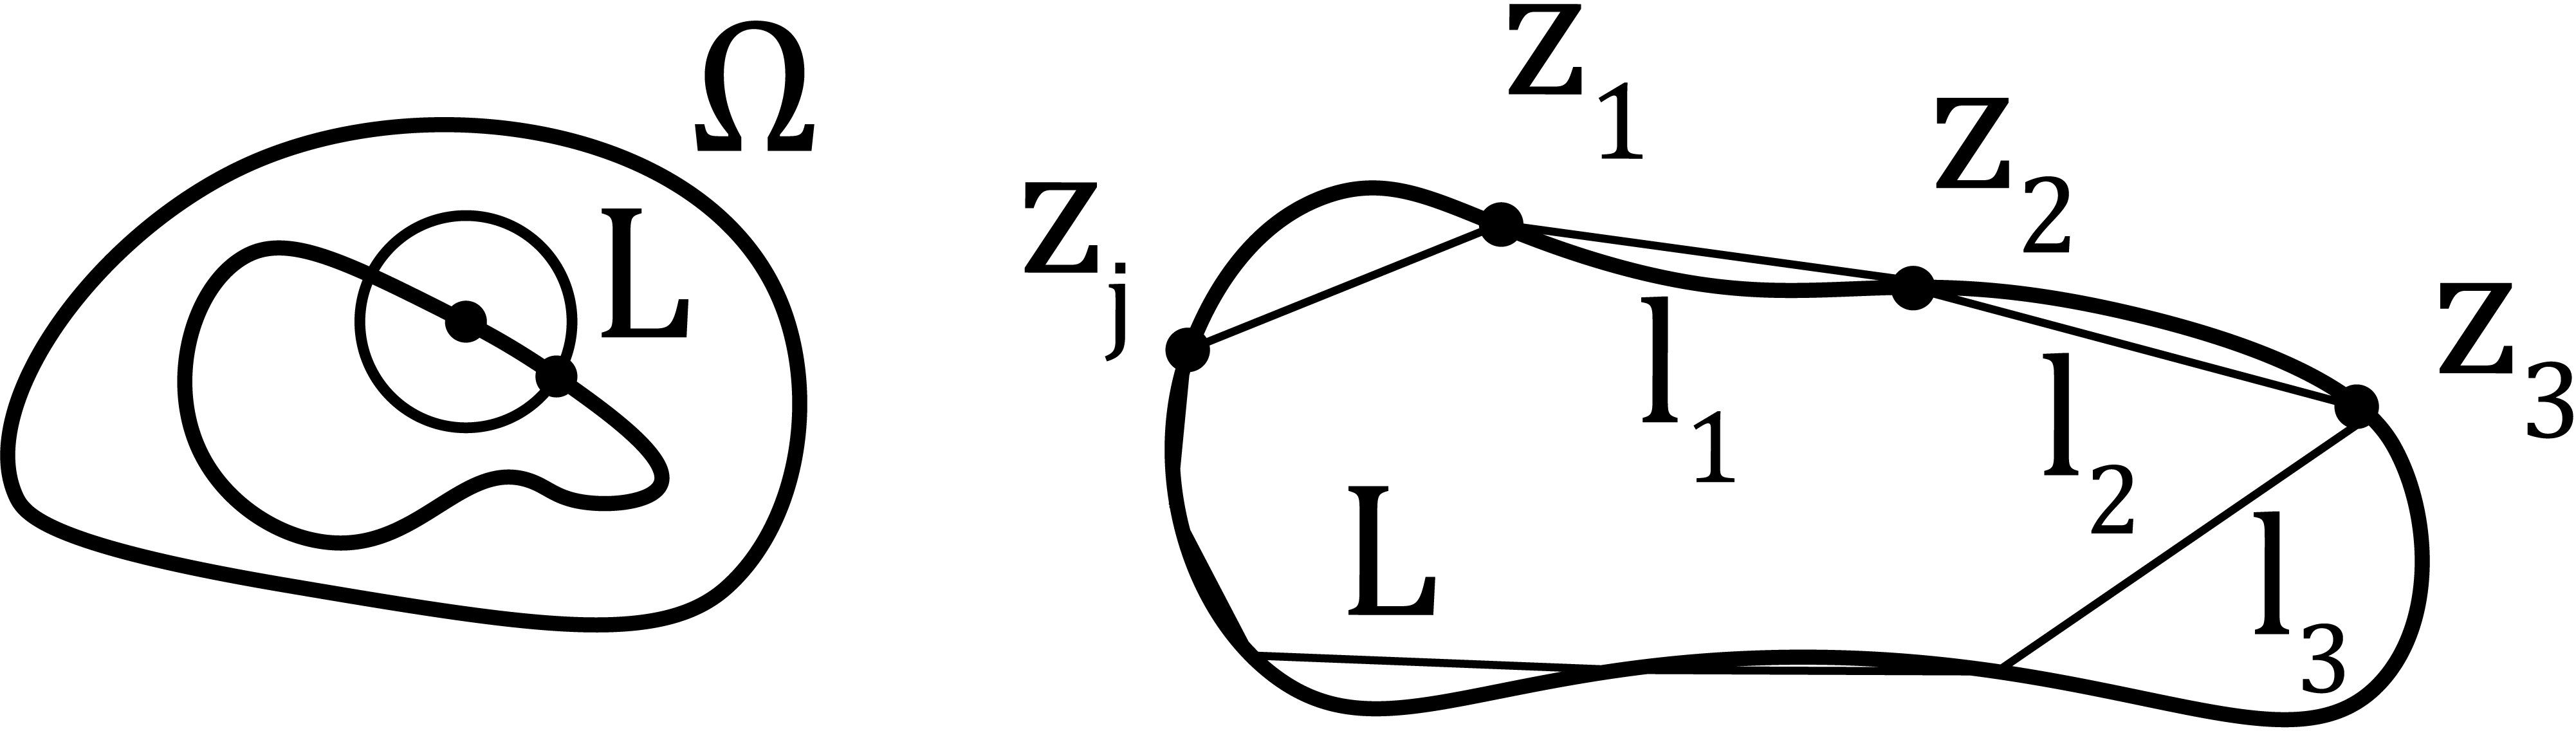
\includegraphics[width=2.5cm]{11_8}
        \end{figure}
        \begin{figure}[H]
          \centering
          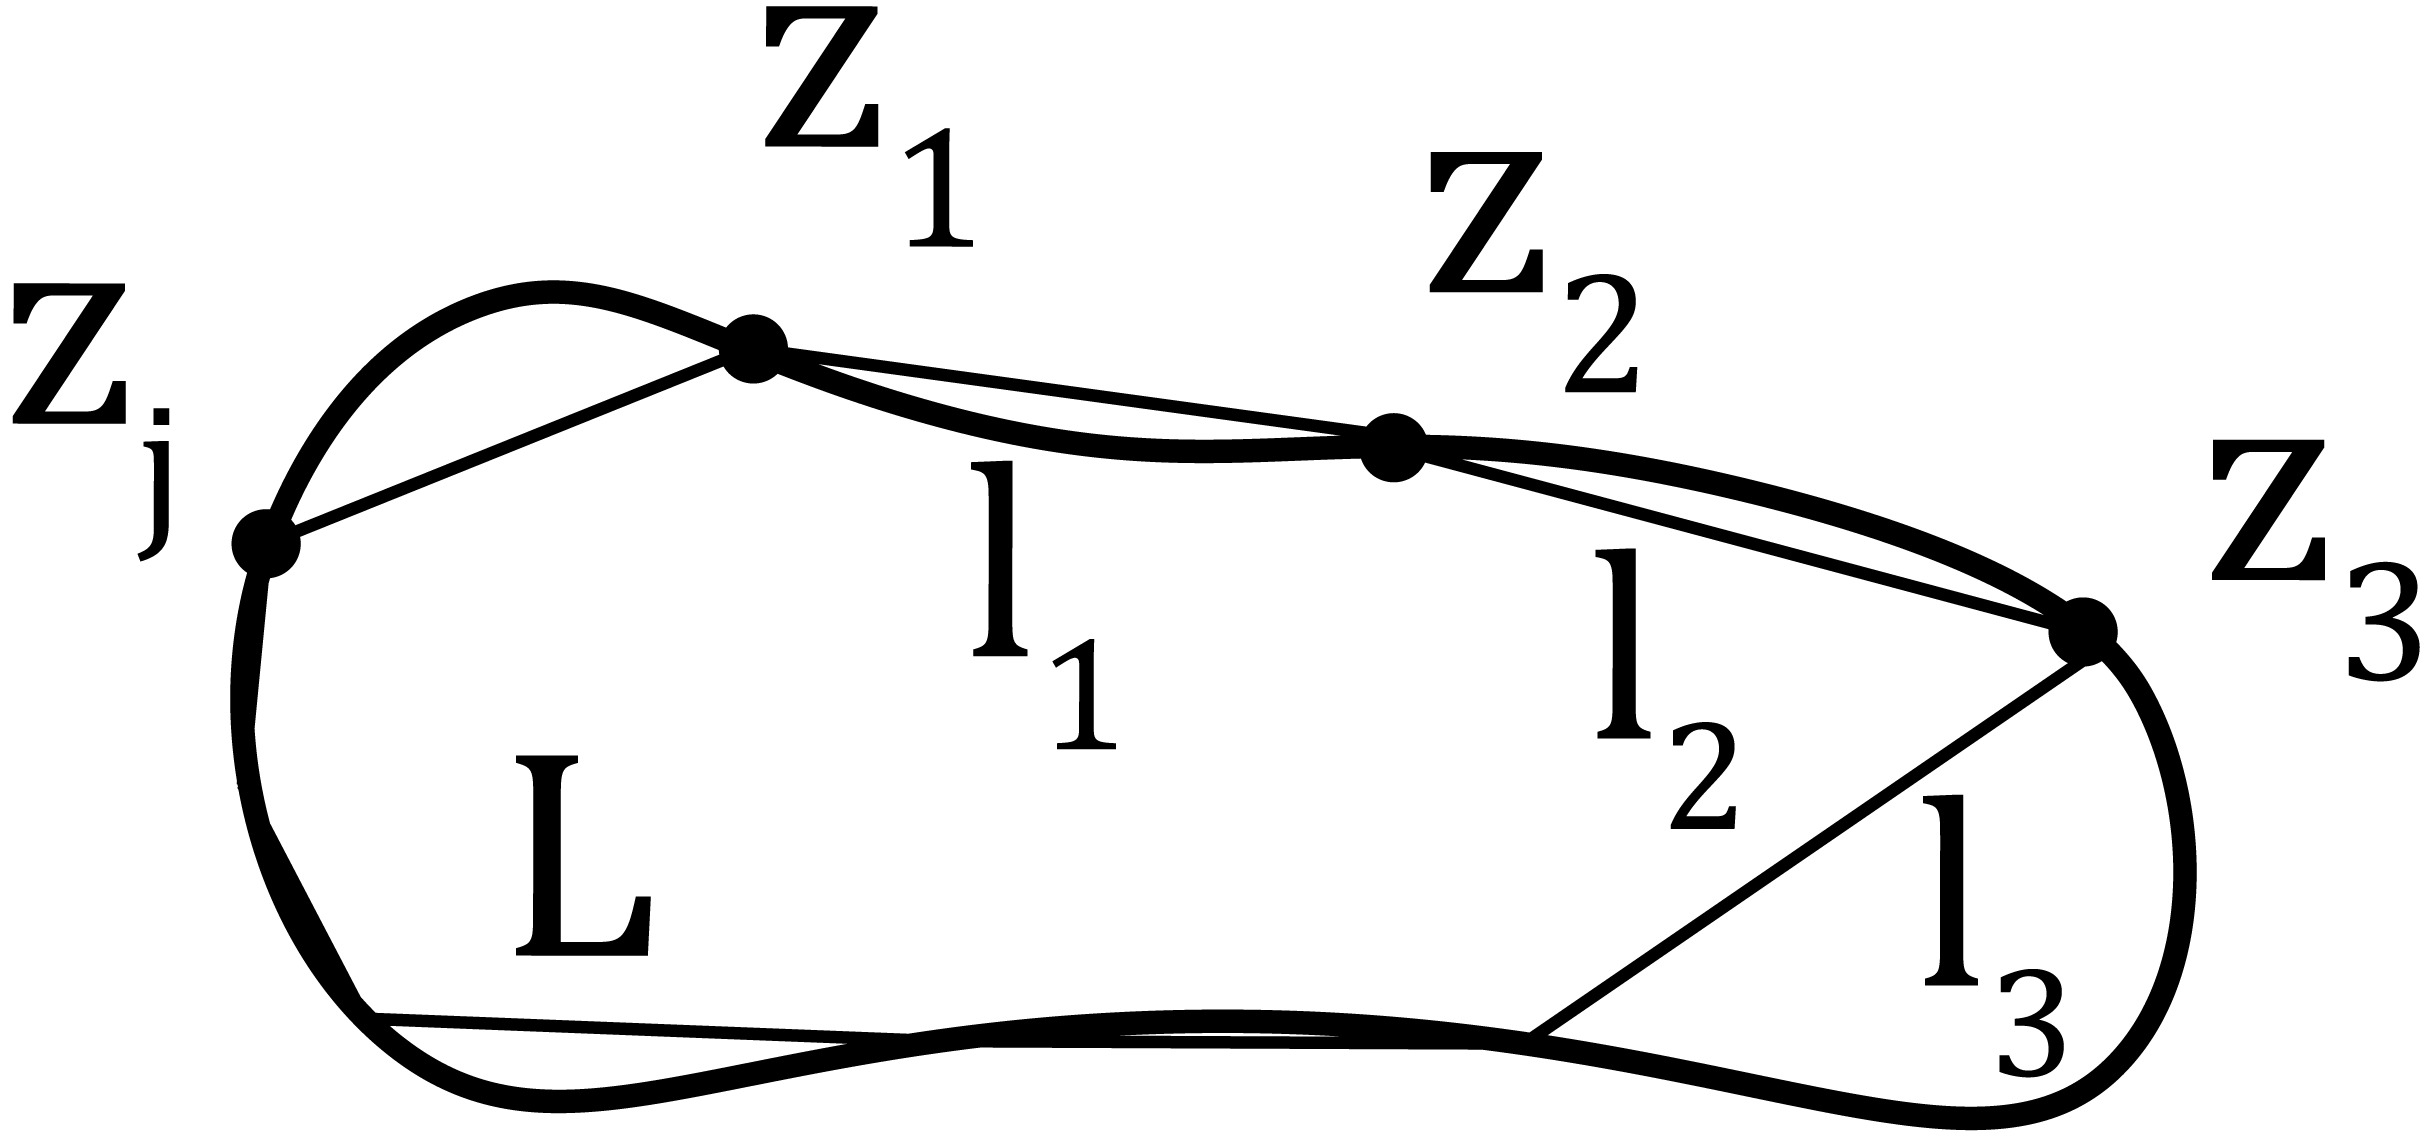
\includegraphics[width=5cm]{11_9}
        \end{figure}
        \[\{z_j\}^N_{j = 1} \text{ - точки на L:} \]
        \[L = \bigcup_{j = 1}^N l_j \]
        \[\us{\text{длина кривой}}{\abs{l_j}} < \delta\]
        \[P \text{ - ломанная, соед } z_j \q P = \cup P_j \q P_j = [z_j, z_{j + 1} ]\]
        \[\int_P f(z)dz = 0 \text{ (по след. из т. Гурса)}\]
        \[\abs{\int_{L} f(z)dz} = \abs{\int_L f(z)dz - \int_P f(z)dz} =
        \abs{\sum_{j = 1}^N \int_{l_j} f(z)dz - \sum_{j = 1}^N  \int_{p_j} f(z)dz  }
        \os{*}{\leq}\]
        \[\leq \sum_{j = 1}^N \abs{\int_{l_j} f(z)dz - \int_{P_j} f(z)dz  } \]
        \[\abs{\int_{l_j} f(z)dz - \int_{P_j} f(z)dz} \leq \]
        \[\abs{l_j} < \delta \Ra \abs{P_j} < \delta\]
        \[\text{dist}(z_j, z) < \delta \qq \forall z \in l_j, P_j\]
        \[\int_{l_j} f(z_j)dz = f(z_j) \int_{l_j}dz = f(z_j) \cdot (z_{j + 1} - z_j )\]
        \[\int_{P_j} f(z_j)dz = f(z_j) \int_{P_j}dz = f(z_j) \cdot (z_{j + 1} - z_j )  \]
        \begin{figure}[H]
          \centering
          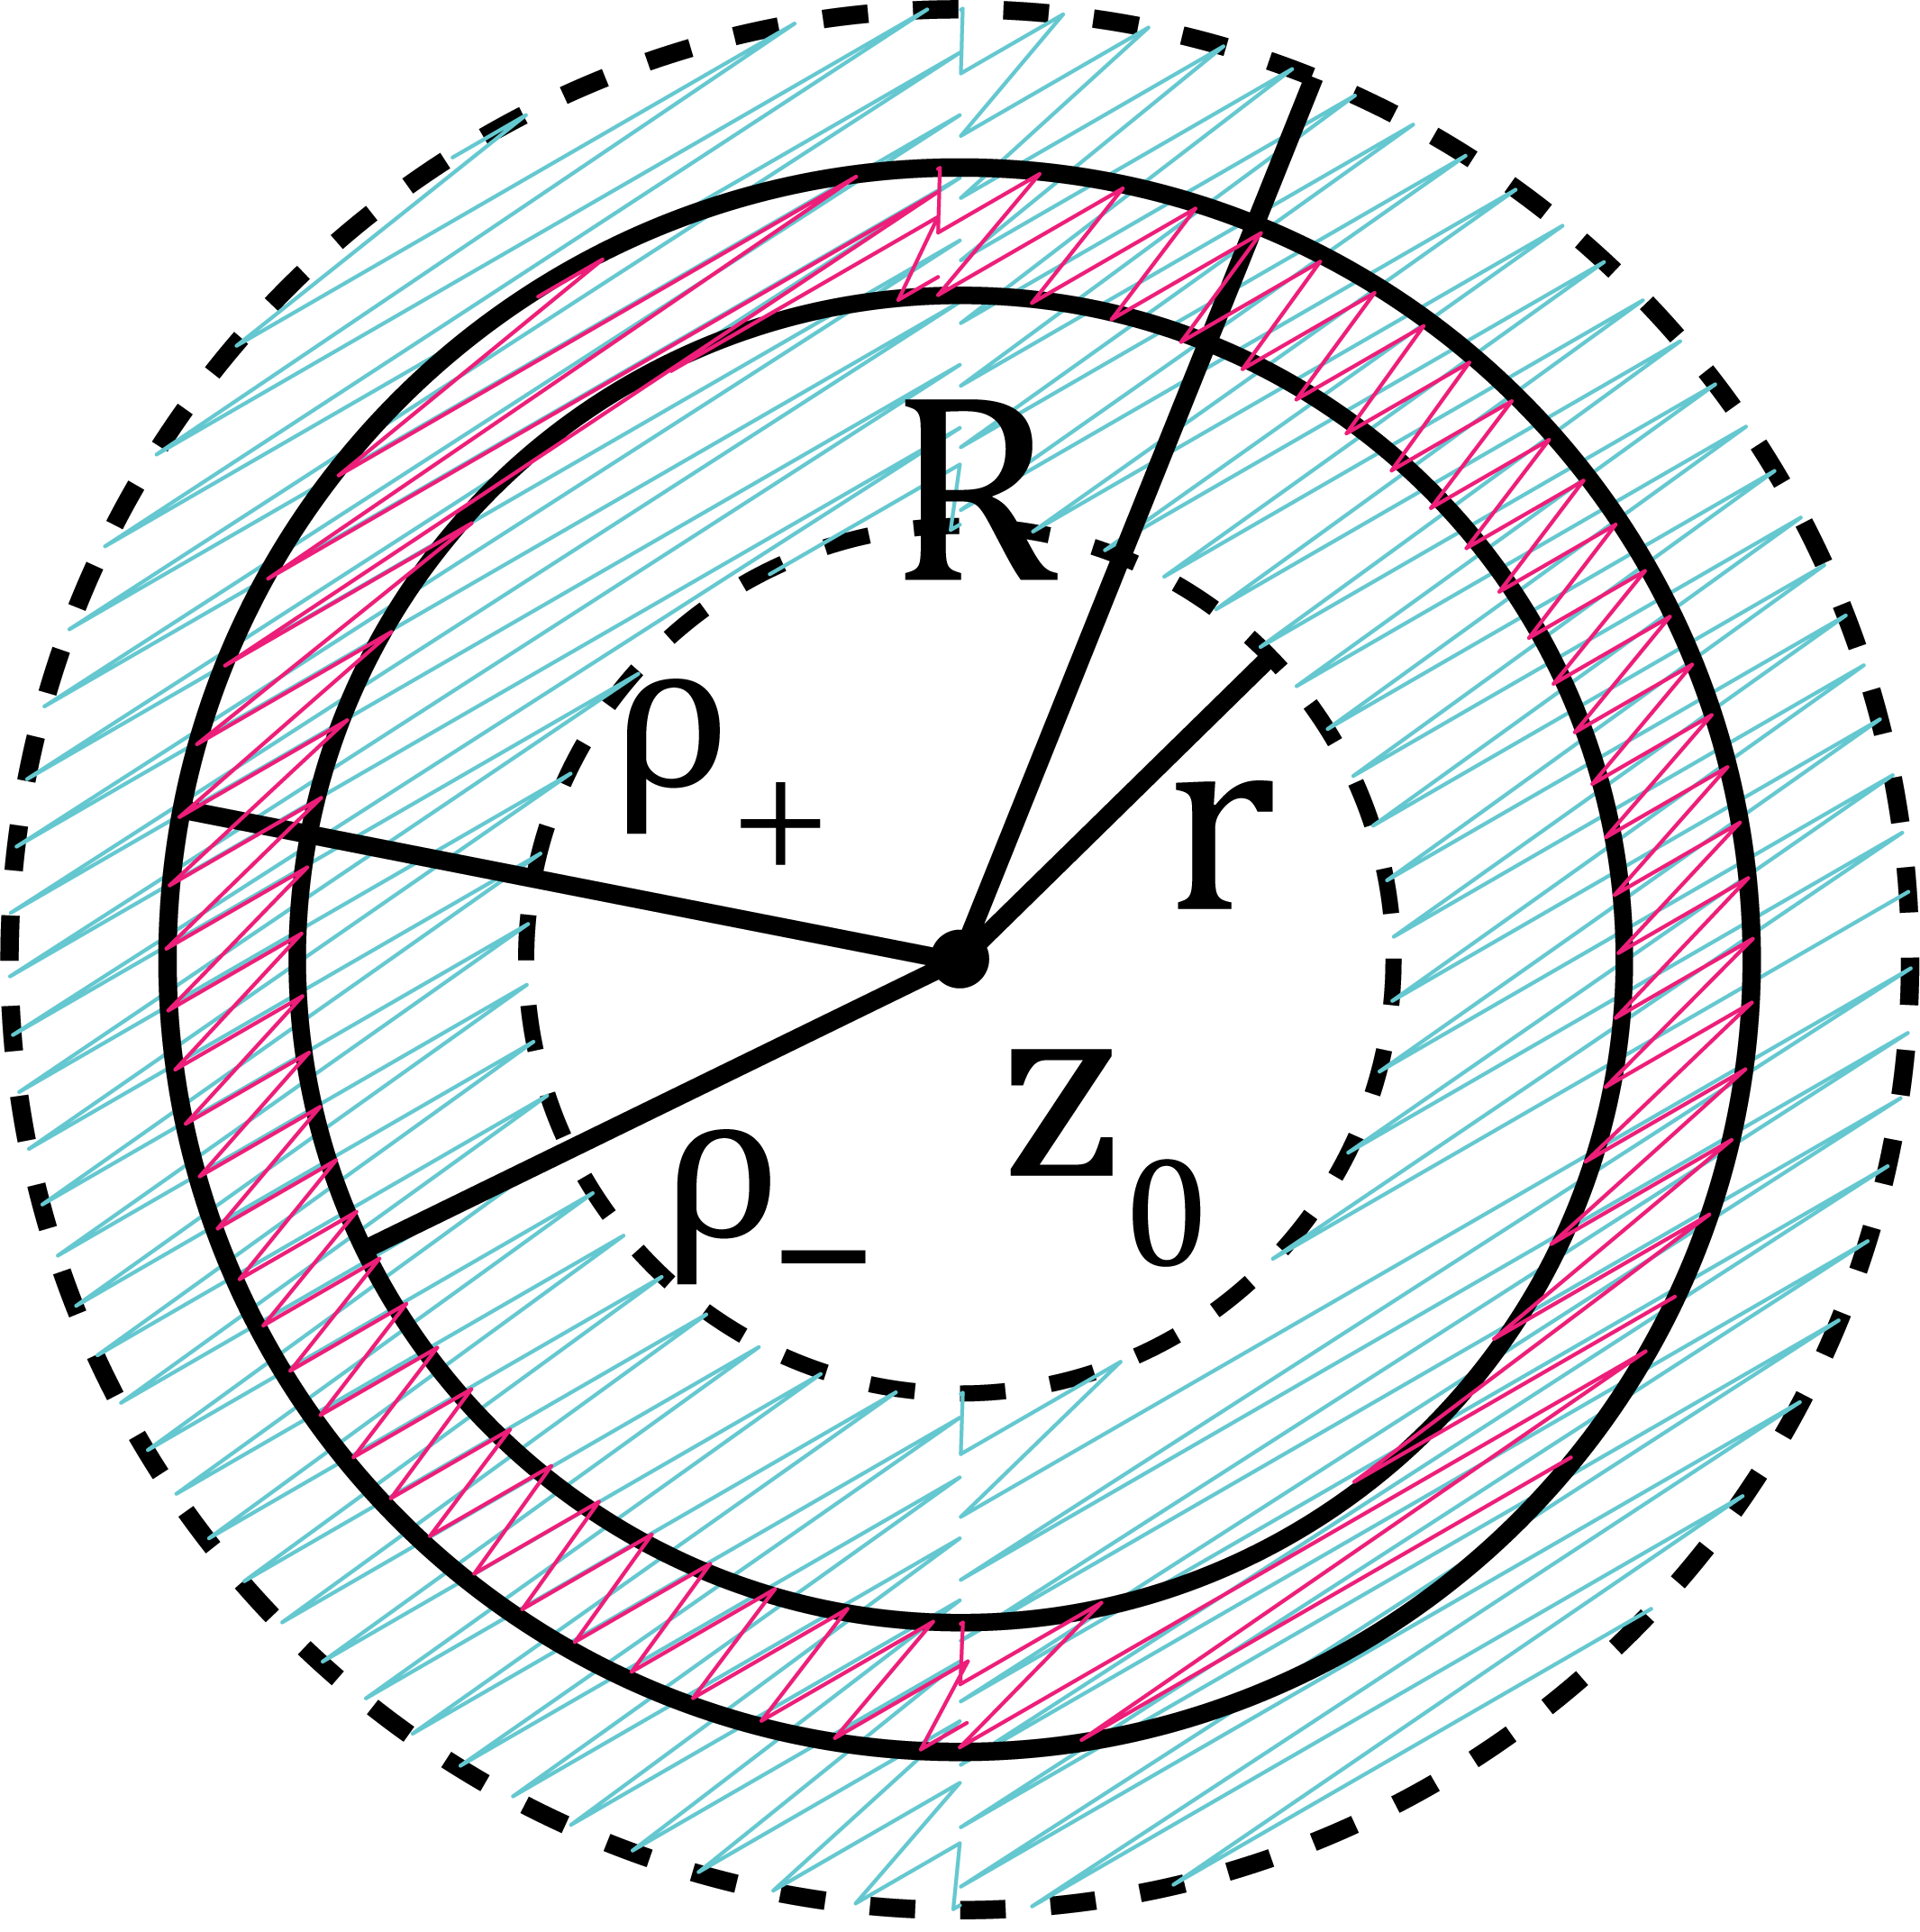
\includegraphics[width=5cm]{11_11}
        \end{figure}
        \[\os{*}{\leq } \abs{\int_{l_j} (f(z) - f(z_j))dz} +
        \abs{\int_{P_j}(f(z) - f(z_j))dz } \leq \max_{z \in l_j} \abs{f(z) - f(z_j)}\cdot
        \abs{l_j} + \]
        \[+ \max_{z \in P_j} \abs{f(z) - f(z_j)} \cdot \abs{P_j} \]
        \[\max < \mathcal{E} (\text{т.к. }  \abs{z - z_j} < \delta)\]
        \[\abs{\int_L f(z)dz} \leq \sum_{j = 1}^N \mathcal{E} \abs{l_j} +
        \mathcal{E}\abs{P_j} = \mathcal{E}(\abs{L} + \abs{P}) \leq 2 \mathcal{E} \abs{L} \]
        т.к. $\mathcal{E}$ - произв. $ \displaystyle \Ra \abs{\int_L f(z)dz} = 0$
    \end{proof}

    \begin{Theorem}[интегральная формула Коши]
        \[L = \d D,\q D \subset \Omega\]
        \[f \text{ - диф-ма } \forall z \in \Omega\]
        \[z_0 \in \Omega \setminus L\]
        \begin{figure}[H]
          \centering
          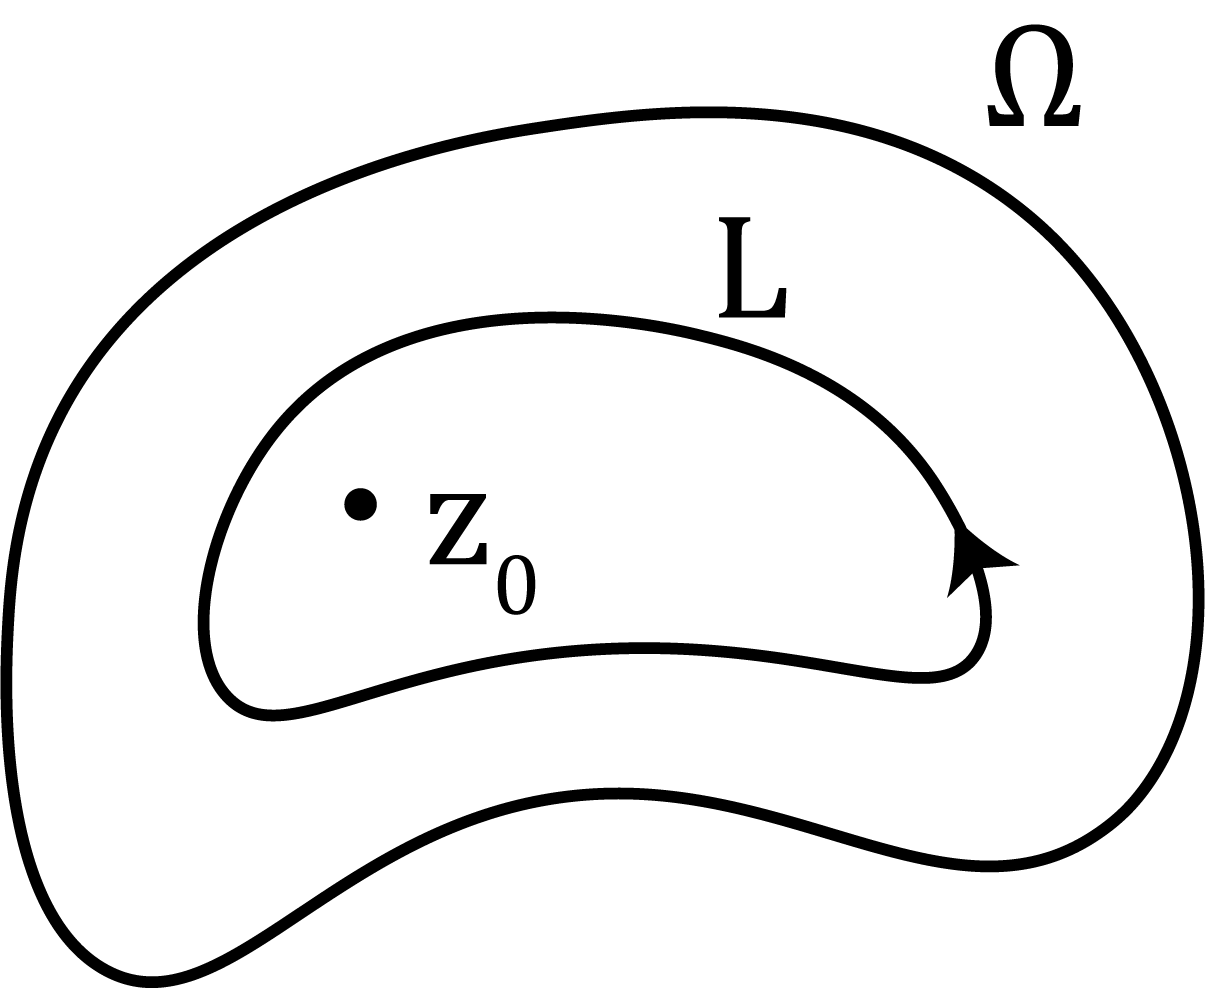
\includegraphics[width=4cm]{11_12}
        \end{figure}
        \begin{figure}[H]
          \centering
          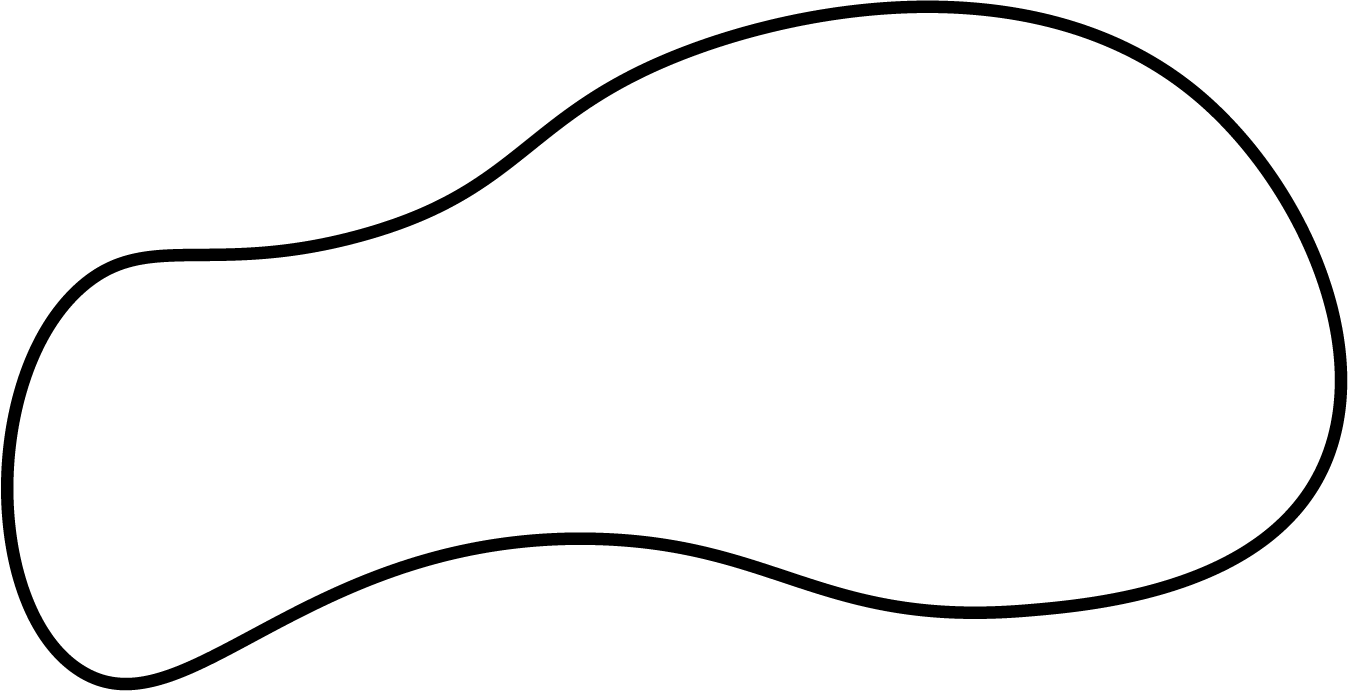
\includegraphics[width=4cm]{11_13}
        \end{figure}
        \[\text{Тогда } \frac{1}{2\pi i}\int_L \frac{f(\xi)}{\xi - z_0}d\xi = \begin{cases}
            f(z_0), & z_0 \in D\\
            0, & z_0 \ \cancel{\in }\ \overline{D}
        \end{cases}\]
    \end{Theorem}

    \begin{Proof}
        \[g(z) = \begin{cases}
            \frac{f(z) - f(z_0)}{z - z_0}, & z \neq z_0\\
            f'(z_0), & z = z_0
        \end{cases}\]
        \[ g \text{ - диф-ма } \forall z \neq z_0, \q z \in \Omega \text{ и  }
        g \in C(\Omega)\]
        \[\text{т.о } g \text{ - удовл. усл. т. Коши } \Ra \int_L g(z)dz = 0 \]
        \[0 = \int_L g(\xi)d\xi = \int_L \frac{f(\xi) - f(z_0)}{\xi - z_0}d\xi =
        \int_L \frac{f(\xi)}{\xi - z_0}d\xi - f(z_0)\int_{L} \frac{d\xi}{\xi - z_0} \]
        \[\int_L \frac{f(\xi)}{\xi - z_0}d\xi = f(z_0)\int_L \frac{d\xi}{\xi - z_0}\]
        \begin{figure}[H]
          \centering
          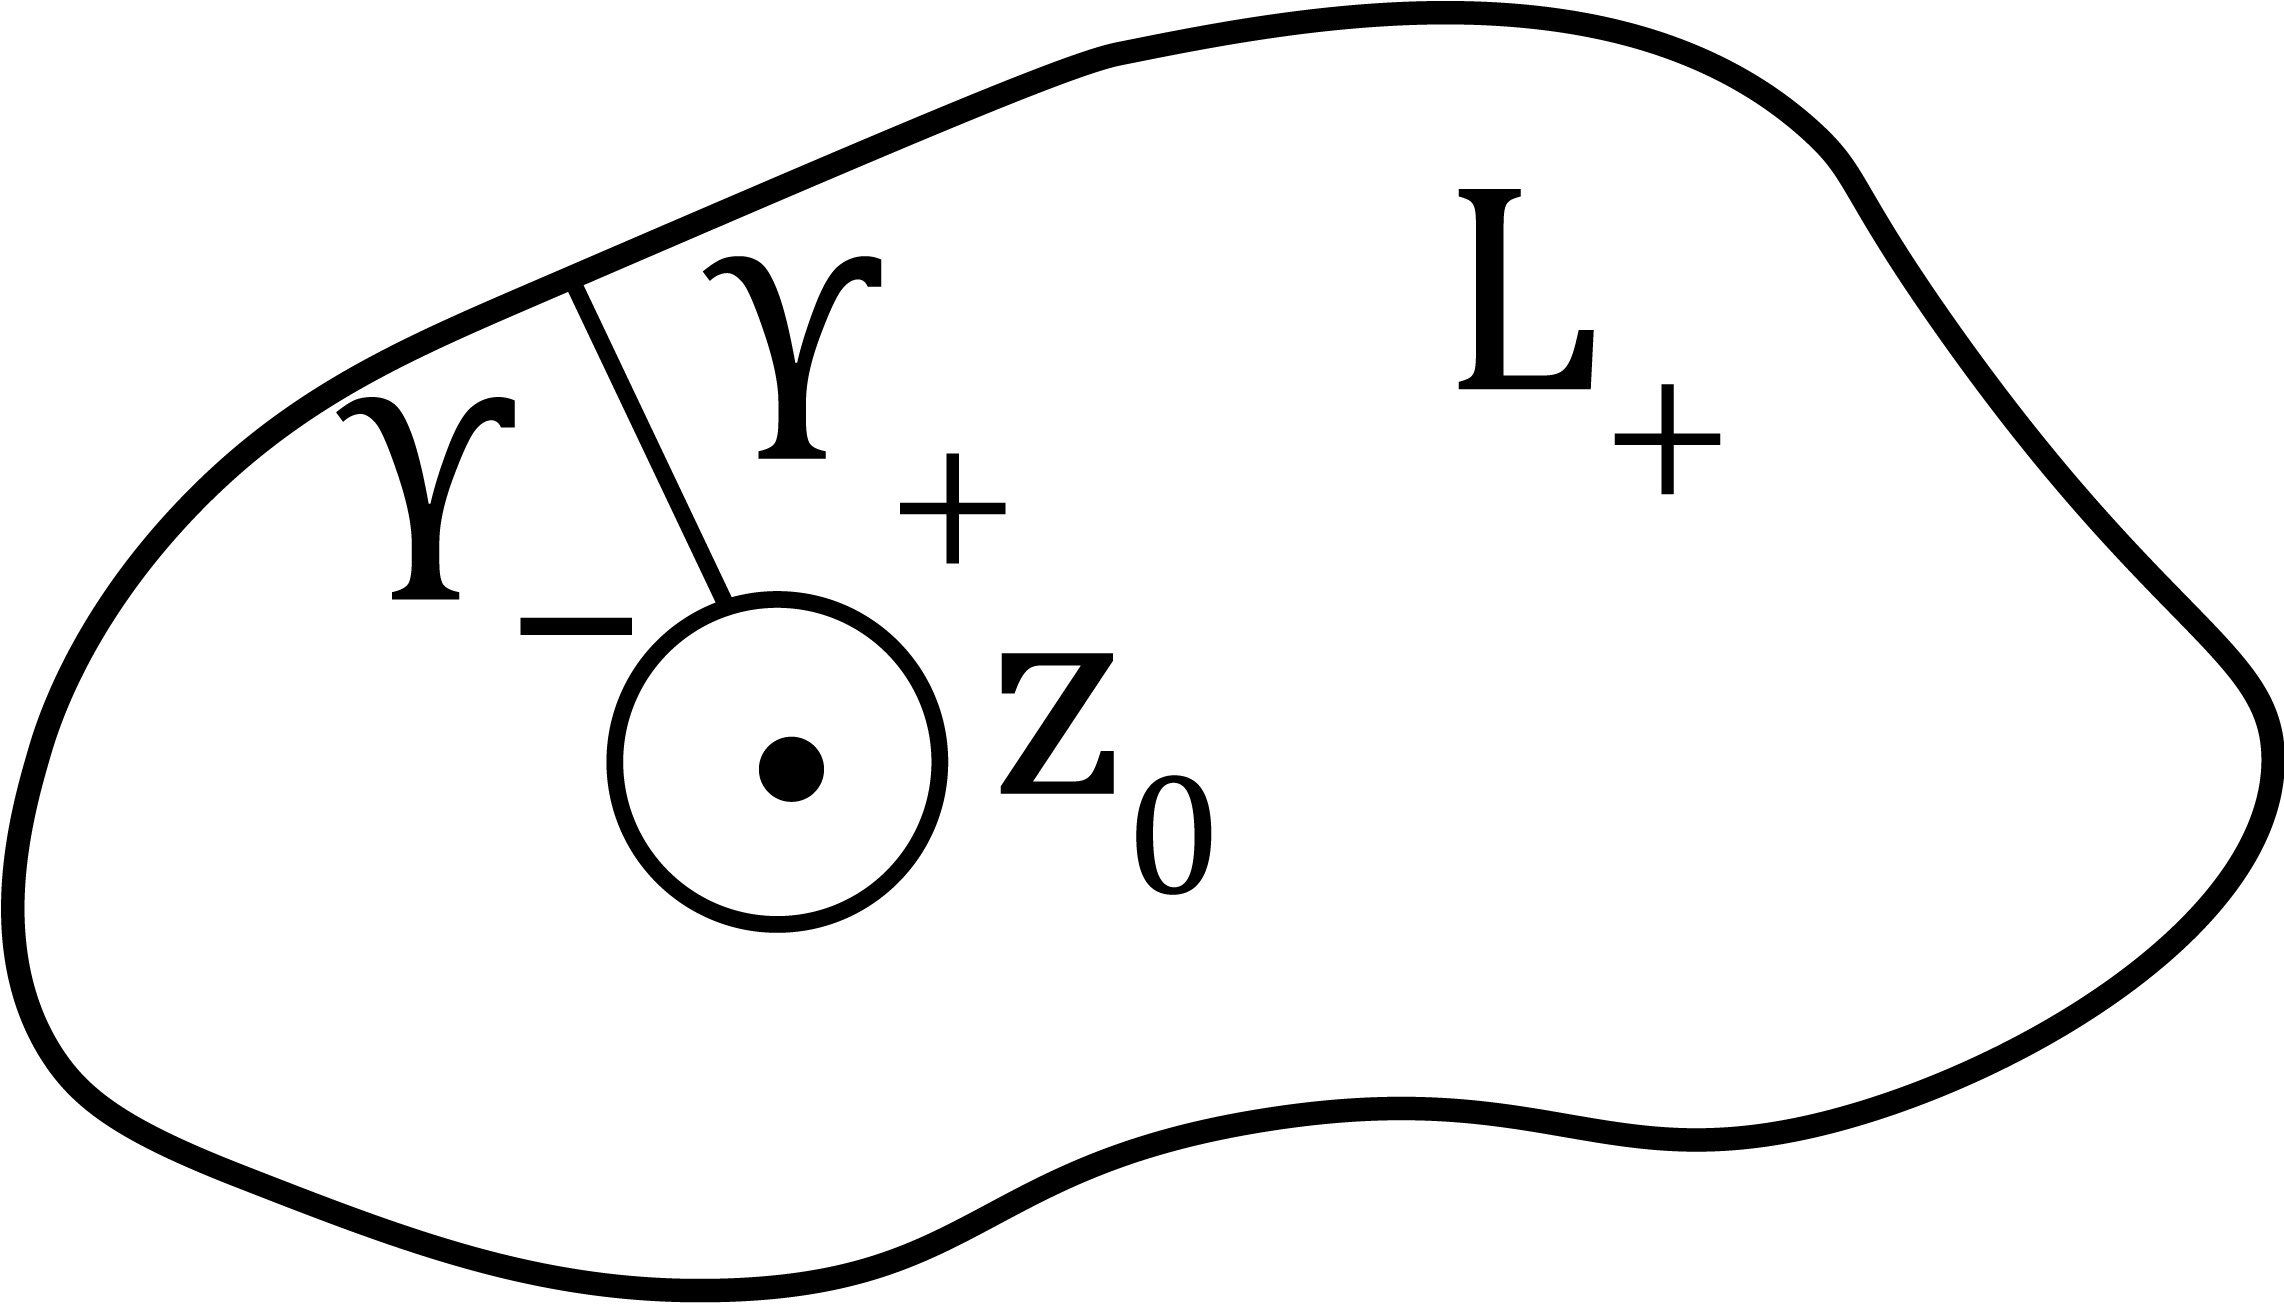
\includegraphics[width=4cm]{11_14}
        \end{figure}
        \[D(z_0, r), \q r < \text{ dist}(z_0, L)\]
        \[\widetilde{L} = L_+ \cup \gamma_+ \cup \gamma_- \delta_r^-\]
        \[\delta_r^- \text{ - граница }D(z_0, r) \text{ по час. стрелке}\]
        \[0 = \int_{\widetilde{L}}  = \int_{L^+} + \int_{\gamma^+} + \int_{\gamma^-} +
        \int_{\delta_r^-} = \int_{L^+} - \int_{\delta^+_r} \]
        \[\int_{L^+} \frac{d\xi}{\xi - z_0} = \int_{\delta^+_r} \frac{d\xi}{\xi - z_0} = 2\pi i\]

        \[\xi = z_0 + re^{it} \]
        \[\text{Если } z_0\ \cancel{\in }\ D \q \frac{f(\xi)}{\xi - z_0} \text{ - диф-ма }
        \forall \xi \in \Omega \setminus \{z_0\}\]
        \[L = \d D\]
        \begin{figure}[H]
          \centering
          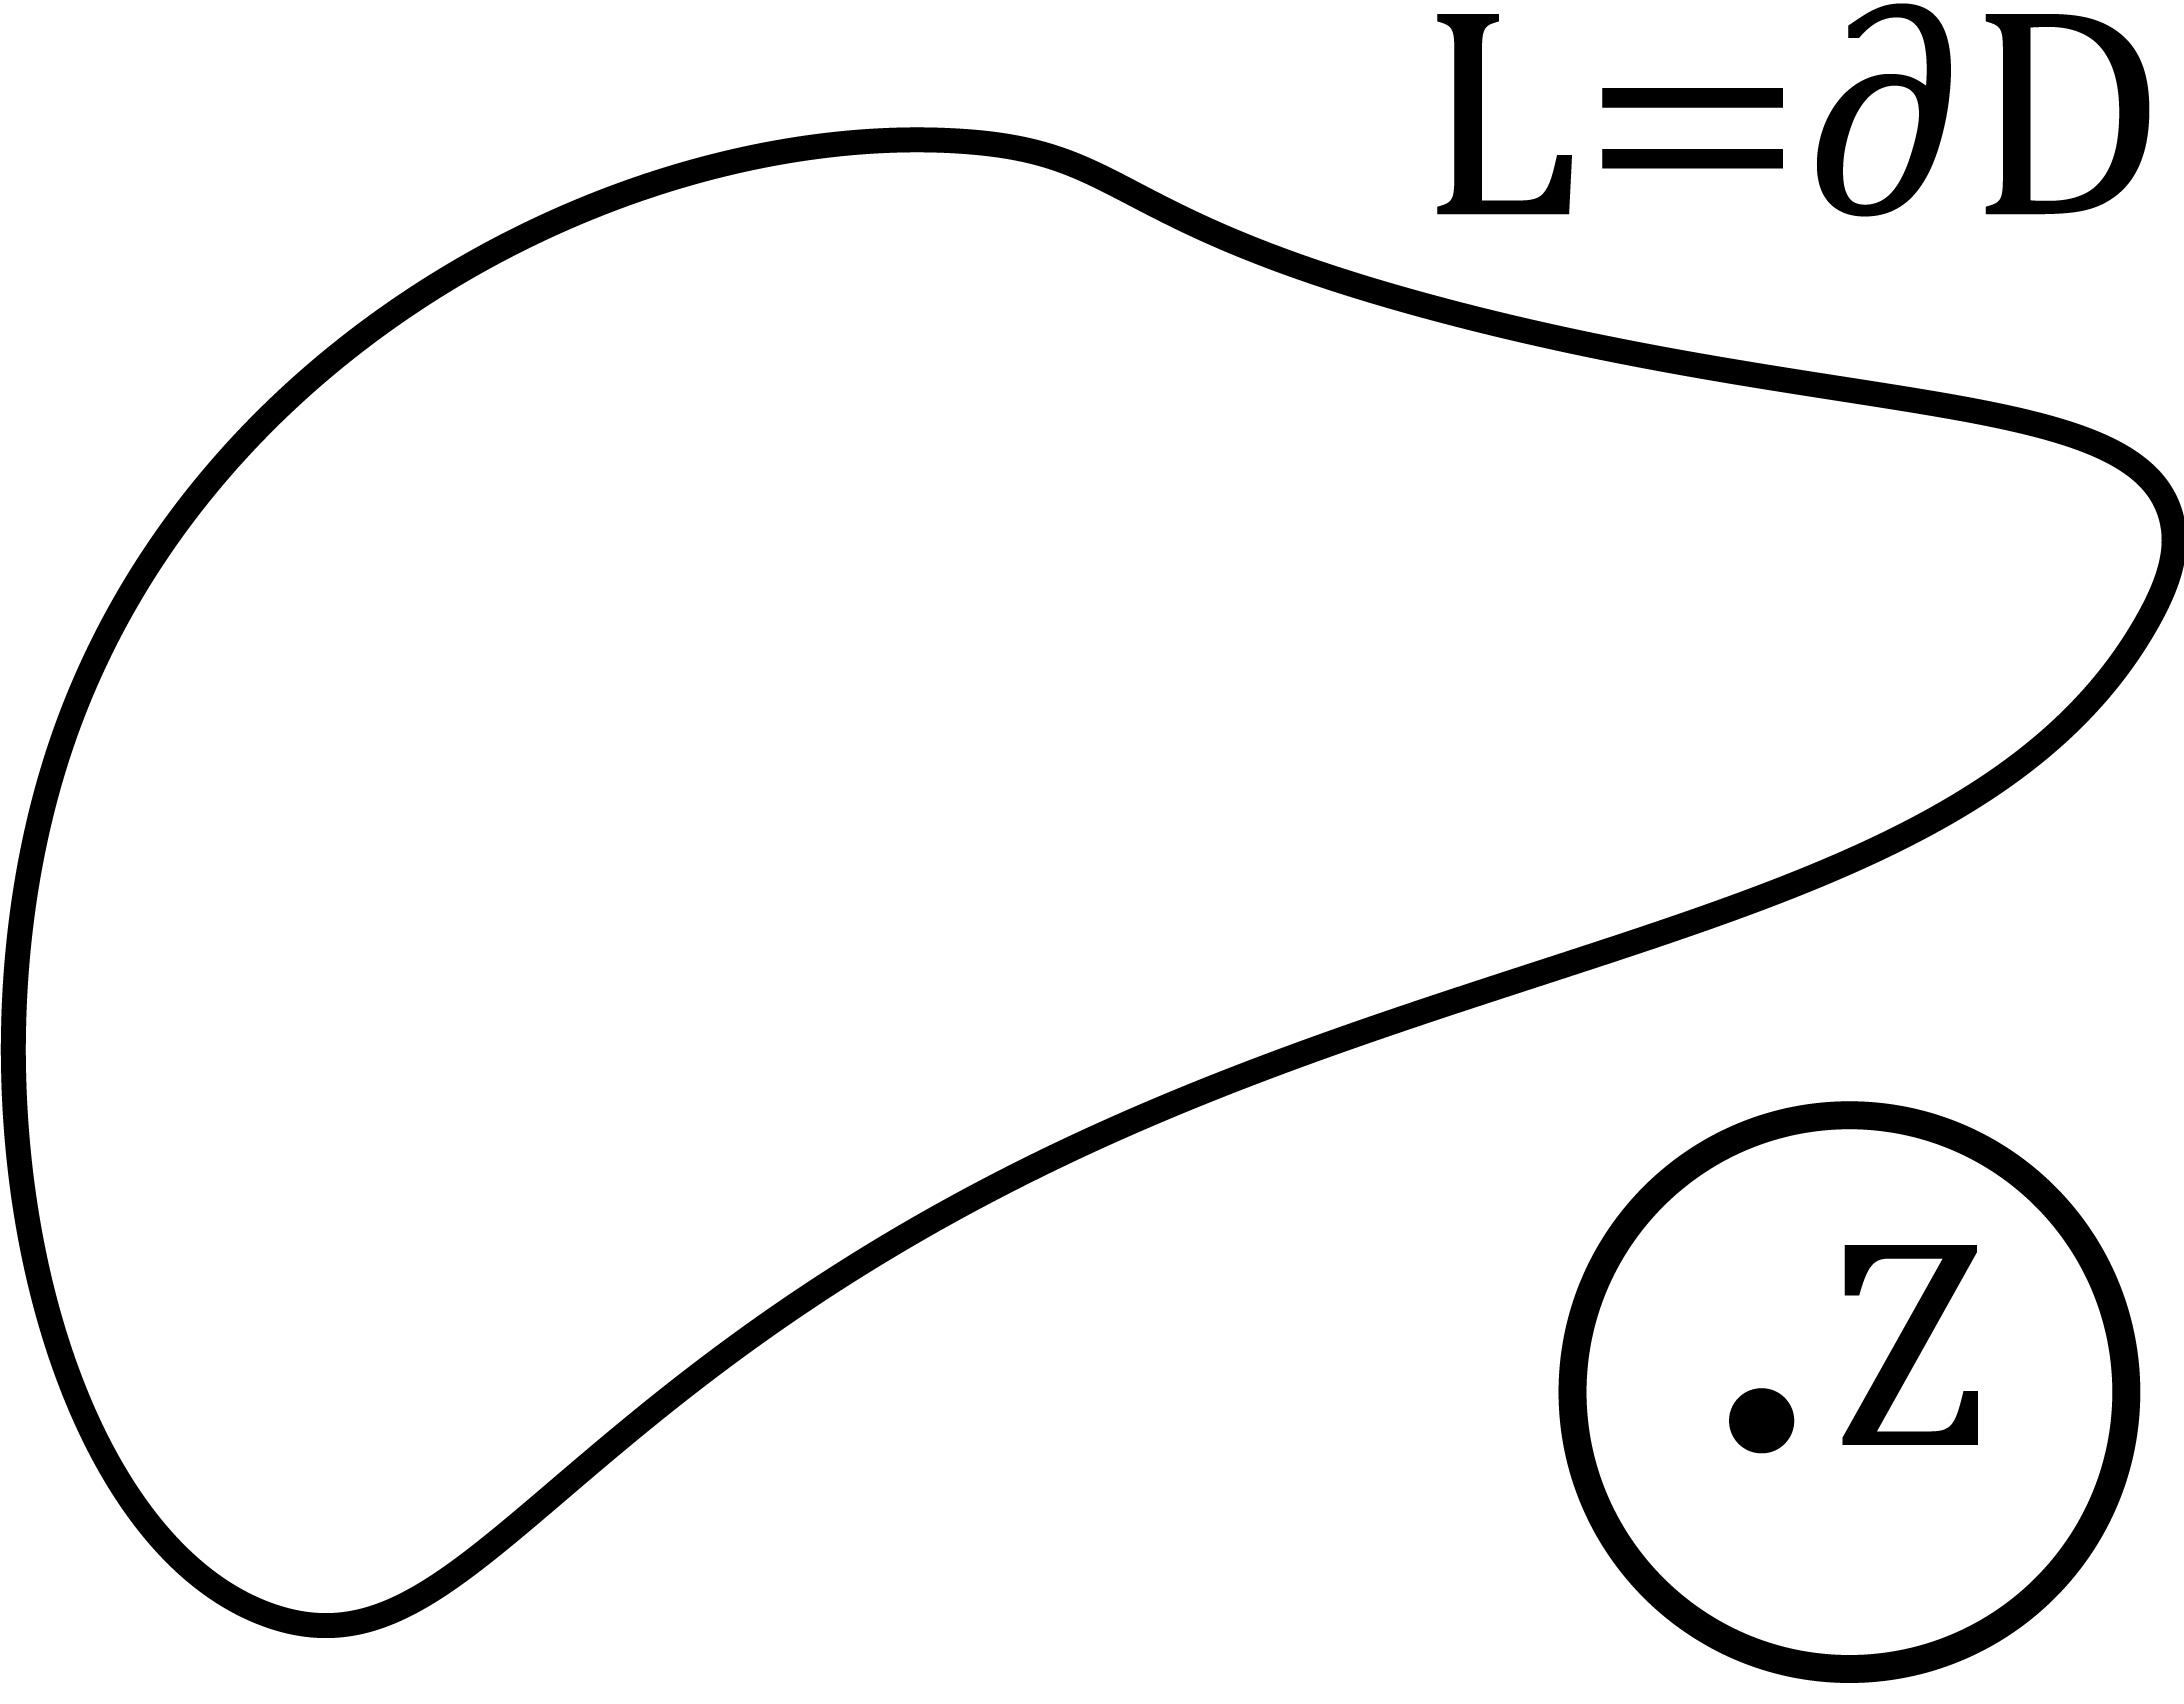
\includegraphics[width=3cm]{11_15}
        \end{figure}
        \[L \text{ вместе с внутр. (т. е. с $D$)}\]
        \[\overline{D} \subset \Omega \setminus \{z_0\}\]
    \end{Proof}

    \begin{Theorem}[Коши о сост. контуре]
        \[L_1, ..., L_p \text{ - простые замк. кривые, не пересек:}\]
        \begin{figure}[H]
          \centering
          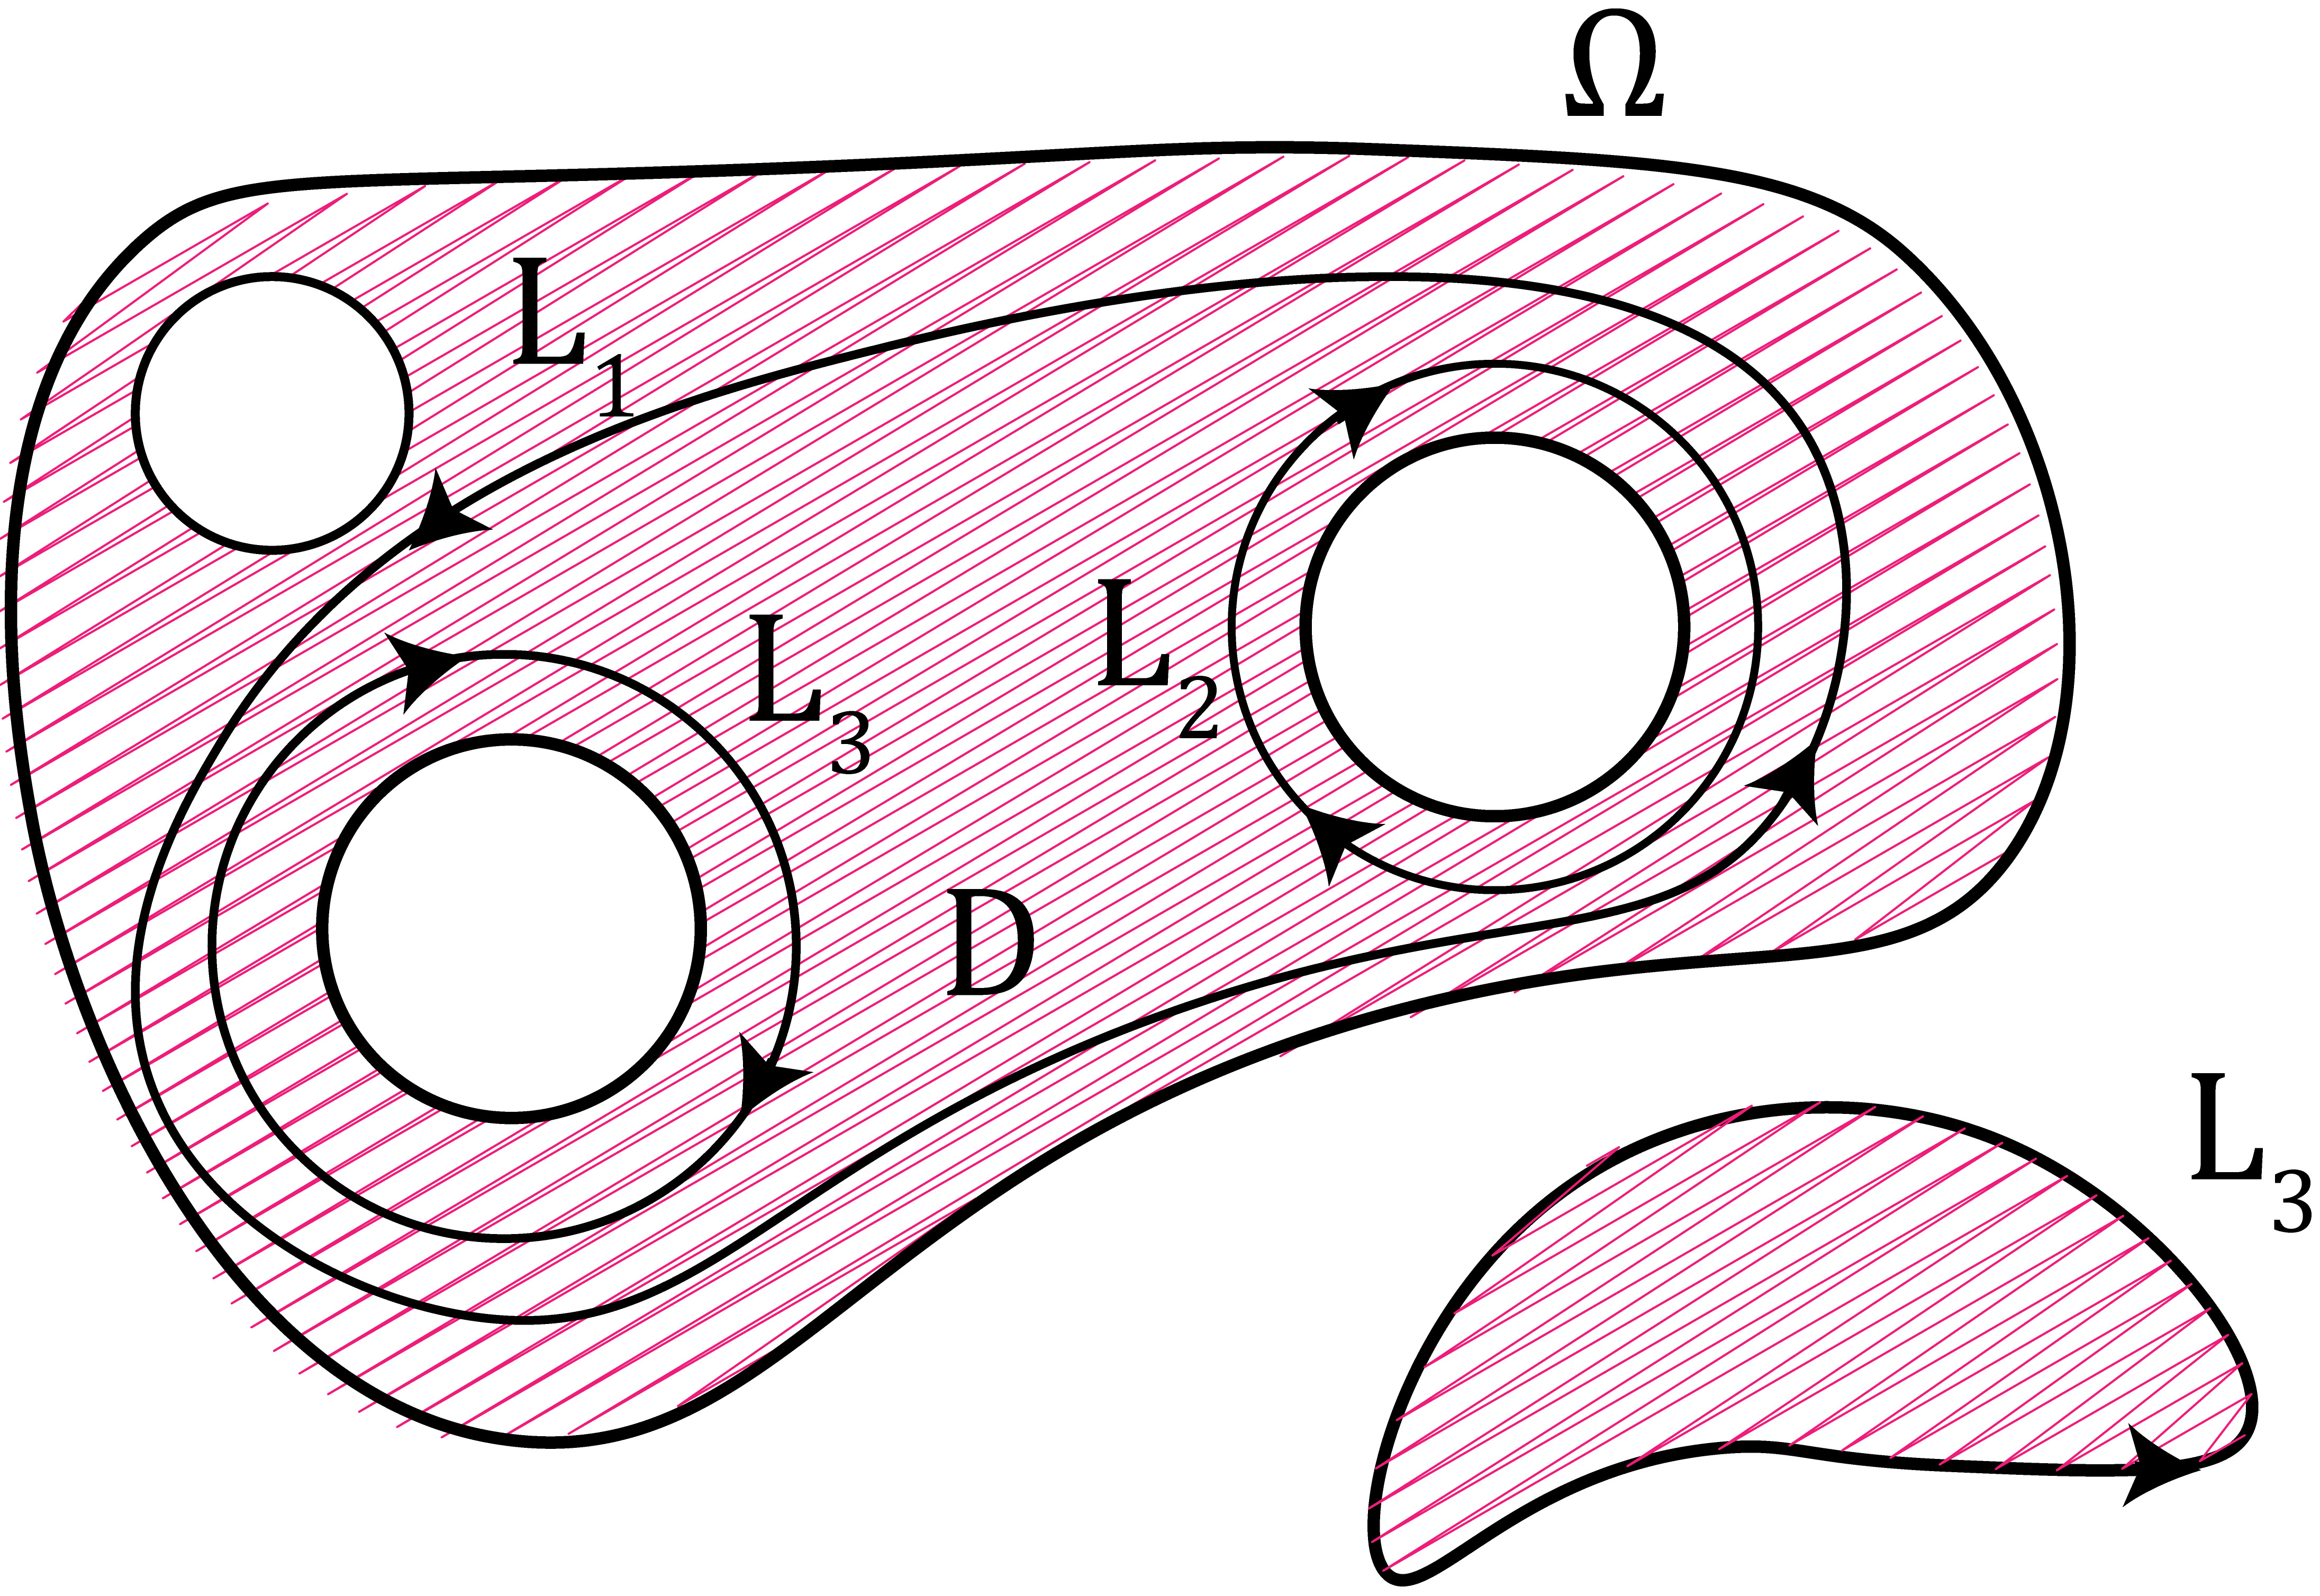
\includegraphics[width=6cm]{11_16}
        \end{figure}
        \[\d D = \bigcup_{j = 1}^P L_j \text{ - сост. контур} \]
        Ориентация $L_j$: при обходе вдоль $L_j$\q $D$ остается слева
        \[f \text{ - диф-ма в } \forall z \in  \Omega \setminus \{p\} \qq z \in C(\Omega) \]
        \[\text{Тогда } \int_{L} f(z)dz = 0 \]
    \end{Theorem}

    \begin{Proof}[P = 2]\
        \begin{figure}[H]
          \centering
          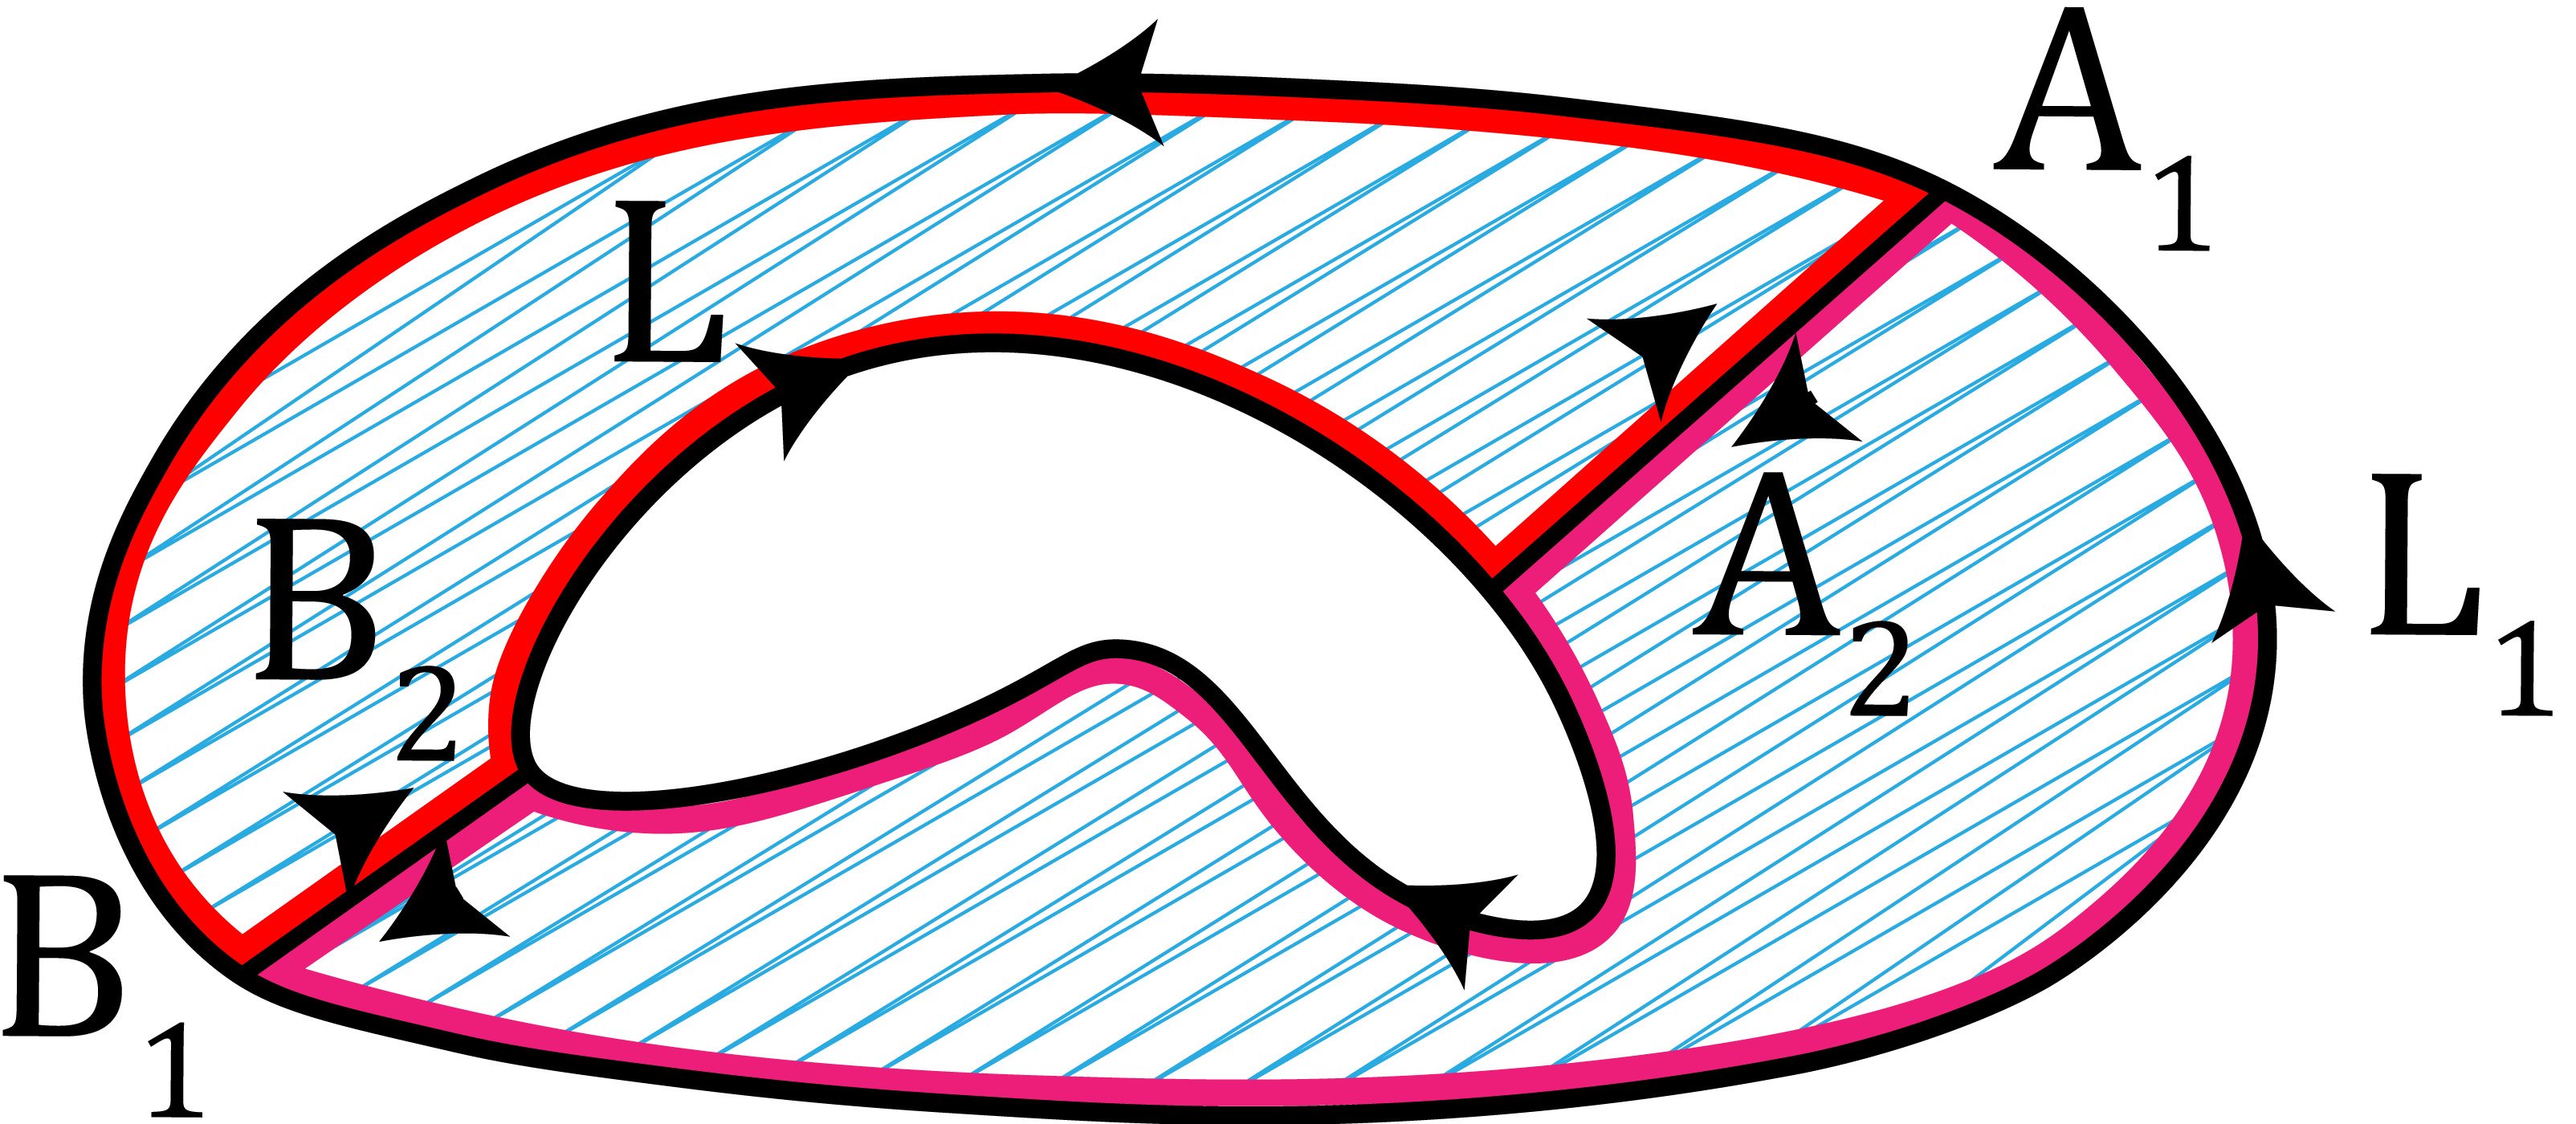
\includegraphics[width=5cm]{11_17}
        \end{figure}
        \[\Gamma_1 = \gamma_{A_1, A_2} \cup L_2^{A_2 B_2}
        \cup \gamma_{B_2 B_1} \cup L_1^{B_1 A_1}    \]
        \[\int_{\Gamma_1} f(z)dz = 0\]
        \[\Gamma_2 = L_1^{A_1 B_1} \cup \gamma_{B_1 B_2} \cup L_2^{B_2 A_2} \cup
        \gamma_{A_2 A_1} \]
        \[\int_{\Gamma_2} f(z)dz = 0 \]
        \[0 = \int_{\Gamma_1} + \int_{\Gamma_2} = \int_{\gamma_{A_1 A_2} } +
        \int_{L_2^{A_2 B_2} } + \int_{\gamma_{B_2 B_1} } + \int_{L_1^{B_1 A_1} } + \]
        \[\int_{\gamma_{A_2 A_1} } + \int_{L_2^{B_2 A_2} } + \int_{\gamma_{B_1 B_2} } +
    \int_{L_1^{A_1 B_1} } = \]

    \[= \int_{L_1 \text{ против ч. стр}} + \int_{L_2 \text{ по час. стр.}} = \int_L f(z)dz  \]
    \end{Proof}

    \begin{Definition} [гармонические функции]
        \[u(x, y) \qq u: D \to \R, \qq D \subset \R^2\]
        \[u \text{ - гармоническая в } D \text{, если }\]
        \[u \in C^2(D)\q \text{ и }\q \frac{\d ^2 u}{\d x^2} + \frac{\d ^2 u}{\d y^2} = 0\]
        \[\text{Лапласиан } \Delta = \nabla^2 = \frac{\d ^2}{\d x^2} + \frac{\d ^2}{\d y^2}\]
        \[\Delta u = 0\]
    \end{Definition}

    \begin{Example}
        \[\text{Пусть } f \in H(\Omega) \qq f \in C^2(\Omega) \text{ потом увидим, что
        не нужно}\]
        \[\Ra u, v \in C^2 (\Omega)\]
        \[f = u + iv \qq u : \Omega \to \R \qq v : \Omega \to \R \qq \Omega \subset \R^2\]
        \[\Ra \begin{cases}
            \frac{\d u}{\d x} = \frac{\d v}{\d y}  & \bigg| \frac{\d }{\d x}\\
            \frac{\d u}{\d y} = - \frac{\d v}{\d x} & \bigg| \frac{\d }{\d y}
        \end{cases}\]
        \[\begin{cases}
            \frac{\d ^2 u}{\d x^2} = \frac{\d ^2 v}{\d y \d x}\\
            \frac{\d ^2 u}{\d y^2} = - \frac{\d ^2 v}{\d x \d y}
        \end{cases}\]
        \[\frac{\d ^2 u}{\d x^2} + \frac{\d ^2 u}{\d y^2} = 0\]
        \[\Ra u \text{ - гармонич.}\]
        Аналогично
        \[\frac{\d ^2 v}{\d x^2} + \frac{\d ^2 v}{\d y^2} = 0\]
        \[v \text{ - тоже гармонич.}\]
        С другой стороны, если $u$ - гармонич.\\
        то $\exists f$ - аналитическая: \ $\real f = u$ ?\\
        (потом)
        %\[\exists ? v \text{ - гармонич. }: u + iv = f \]
    \end{Example}

    \begin{Theorem}[о среднем (для аналит. функции)]
        \[f \in H(\Omega)\]
        \begin{figure}[H]
          \centering
          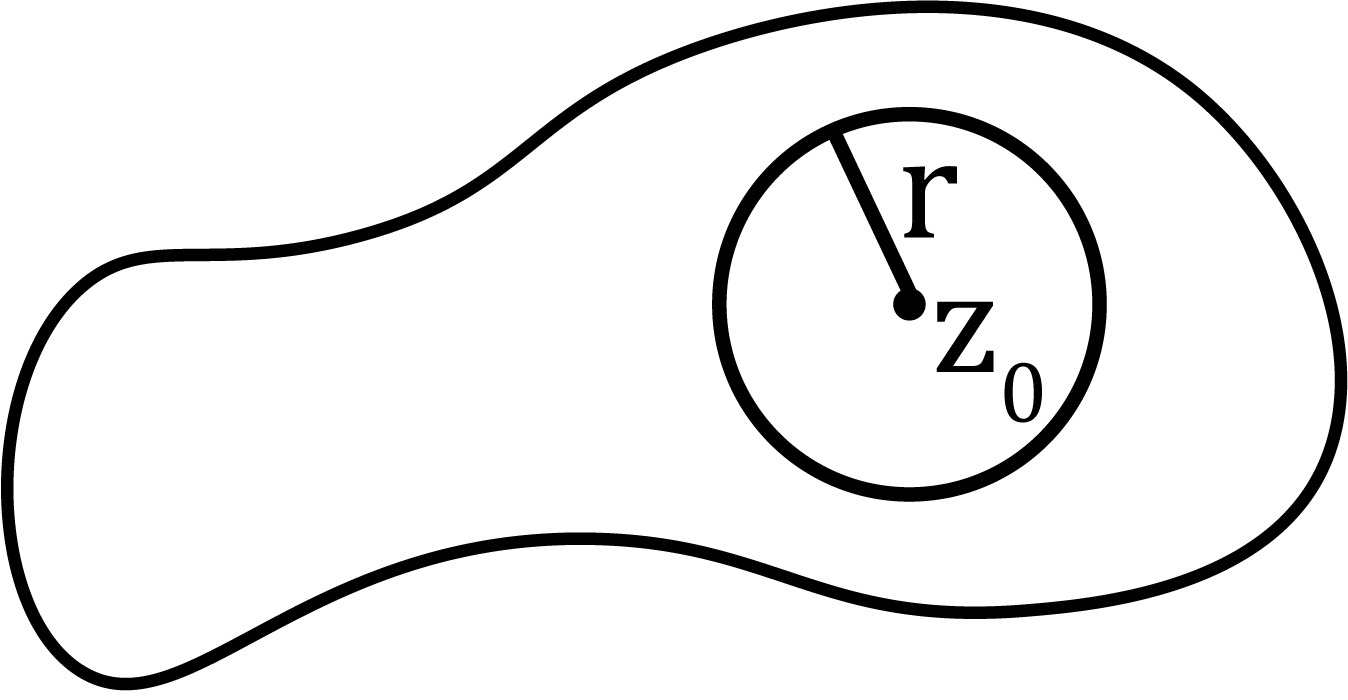
\includegraphics[width=5cm]{11_18}
        \end{figure}
        \[z_0 \in \Omega\]
        \[\overline{D} (z_0, r) \subset \Omega \]
        \[\gamma_r : \xi = z_0 + r\cdot e^{it} \qq 0 \leq t \leq 2\pi \]
        \[\text{Тогда } f(z_0) = \frac{1}{2\pi} \int_{0}^{2\pi} f(z_0 + re^{it} )dt  \]
    \end{Theorem}

    \begin{Proof}
        \[\text{по инт. ф-ле Коши} f(z_0) = \frac{1}{2\pi i} \int_{\gamma_r}
        \frac{f(\xi)}{\xi - z_0} d\xi = \frac{1}{2\pi i }\int_0^{2\pi} \frac{f(z_0 +
        r e^{it} )}{r e^{it} } r i e^{it} dt = \]
        \[= \frac{1}{2\pi}\int_0^{2\pi}  f(z_0 + re^{it} )dt\]
    \end{Proof}

    \begin{consequence}
        В усл. теоремы пусть $f = u + iv$, тогда $u, v$ - гарм. функции
        \[u(z_0) = \frac{1}{2\pi} \int_0^{2\pi} u(z_0 + re^{it} )dt \]
        \[v(z_0) = \frac{1}{2\pi} \int_0^{2\pi} v(z_0 + re^{it} )dt\]
    \end{consequence}

    \subsection{Интеграл и первообразная}

    \begin{Theorem}
        \[f \in C(\Omega)\]
        Следующие условия равносильны
        \begin{enumerate}
            \item $\forall $ замкн $L$ \qq $\displaystyle \int_L f(z)dz = 0$
            \item $\forall \gamma_1, \gamma_2$ с общим началом $A$, общим концом B
                \[\int_{\gamma_1} f(z)dz = \int_{\gamma_2} f(z)dz \]
            \item $\exists F$ - дифф. $\forall z \in \Omega:$
                \[F'(z) = f(z) \qq (\Ra F \in H(\Omega))\]
        \end{enumerate}
    \end{Theorem}

    \begin{Proof}
        \[3 \Ra 2)\]
        \[\int_{\gamma_1} f(z)dz = \int_{\gamma_1} F'(z)dz = F(B) - F(A)  \]
        Аналогично для $\gamma_2$
        \begin{figure}[H]
          \centering
          
\includegraphics[width=3cm]{11_19}
        \end{figure}
        \[2 \Ra 1)\]
        \[\int_L = \int_{L_{AB} }  + \int_{L_{BA} } = 0  \]
        \[1 \Ra 3)\]
        \[z_0 \text{ - зафикс.}\]
        \[F(z) = \int_{z_0}^z f(\xi)d\xi \q \text{ (корректно определена, т.к.
        $\int_{z_0}^{z}  $ не зависит от пути по п.2)}\]
        Проверим дифф-сть.
        \begin{figure}[H]
          \centering
          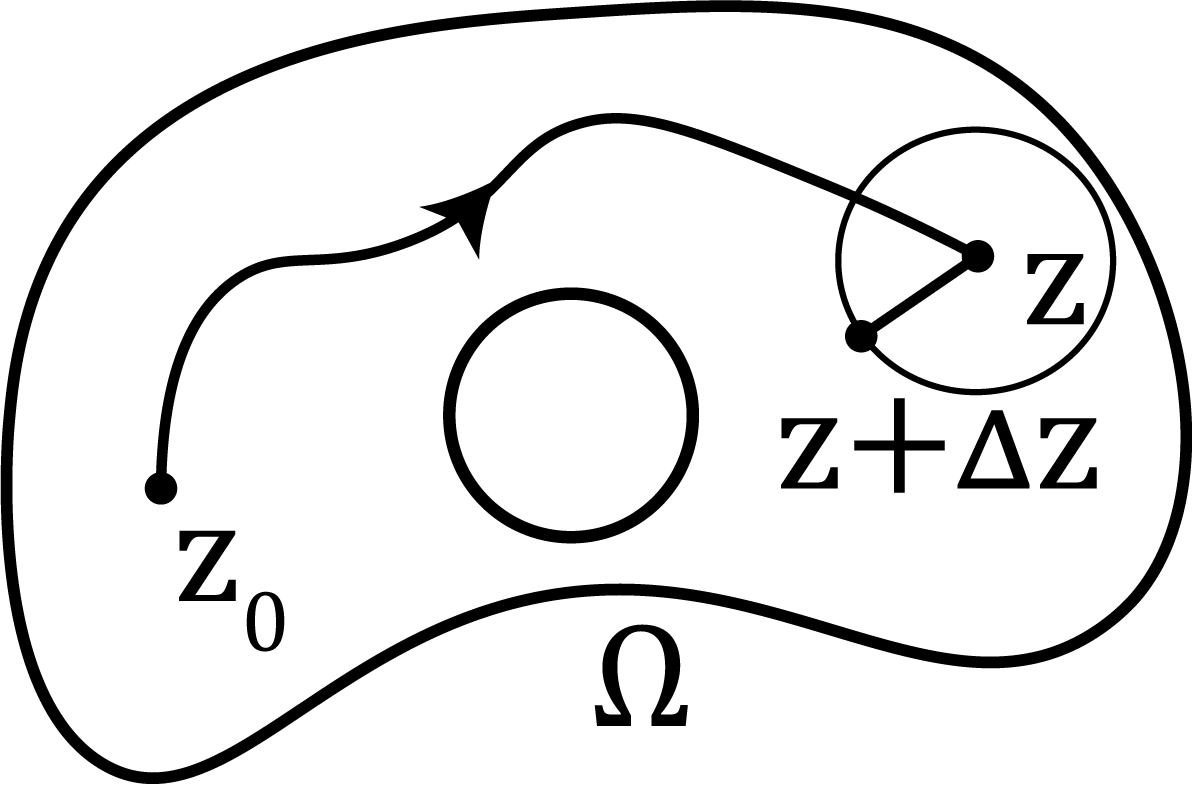
\includegraphics[width=4.5cm]{11_20}
        \end{figure}
        \[\abs{\frac{F(z + \Delta z) - F(z)}{\Delta z} - f(z)} =
       \]
       \[= \abs{\frac{1}{\Delta z} \left[ \int_{z_0}^{z + \Delta z} f(\xi)d\xi -
        \int_{z_0}^{z} f(\xi)d\xi  \right] - \frac{1}{\Delta z} f(z)
        \int_{z}^{z + \Delta z}dz} =\]
        \[= \frac{1}{\abs{\Delta z}} \abs{\int_{z}^{z + \Delta z} (f(\xi) - f(z))d\xi  }
        \os{*}{\leq}\]

        \[f' \text{ - непр в т. } z \Ra \forall \mathcal{E} > 0 \ \exists  \delta :\]
        \[\forall \widetilde{z} : \abs{\widetilde{z} - z} < \delta \ \Ra
        \abs{f(\widetilde{z}) - f(z)} < \mathcal{E}\]
        \[\text{Пусть } \abs{\Delta z} < \delta \q \Ra \q \forall \xi \in [z, z + \Delta z]\]
        \[\abs{\xi - z} < \delta \q \Ra \q \abs{f(\xi) - f(z)} < \mathcal{E}\]

        \[\os{*}{\leq} \frac{1}{\abs{\Delta z}}
        \cdot \mathcal{E} \cdot \abs{[z, z + \Delta z]} = \mathcal{E}\]

        \[\Ra \lim_{\Delta z \to  0} \frac{F(z + \Delta z) - F(z)}{\Delta z} = f(z) \]
        \[\text{т.к. } F \text{ - диф-ма } \forall  z \in \Omega\]
        \[F'(z) = f(z) \in  C(\Omega)\]
        \[F \in H(\Omega)\]
    \end{Proof}

    \begin{reminder}
        Из теории степ. рядов
        \[\sum_{n = 0}^\infty A_n(z - z_0)^n, \q a_n \in \CC \qq z, z_0 \in \CC \]
        Радиус сходимости
        \[R \in [0, +\infty]\]
        \[\frac{1}{R} = \overline{\lim_{n \to \infty } } \sqrt[n]{\abs{a_n}}\]
        \begin{figure}[H]
          \centering
          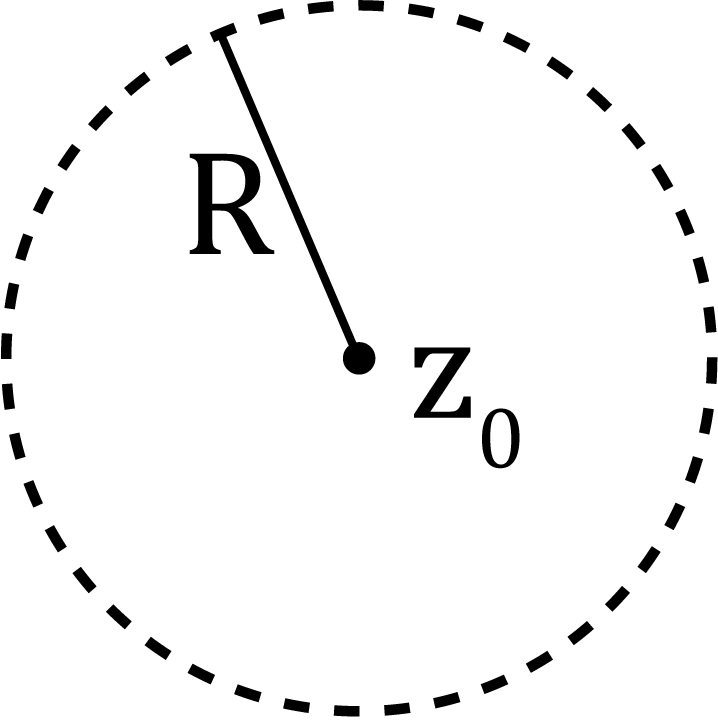
\includegraphics[width=3cm]{11_21}
        \end{figure}
        \[\forall  0 < r < R\]
        Ст. ряд сх. равн. и абс. в $\overline{D}(z_0, r)$
        \[\forall \ z  \ \cancel{\in } \ \overline{D}(z_0, R) \text{ ст. ряд расх.}\]
    \end{reminder}

    \begin{Theorem}[было]
        \[\text{Если } f(z) = \sum_{k = 0}^\infty a_k (z - z_0)^k, \qq R \text{ - рад. сх}\]
        \[z \in D(a, R)\]
        \[\Ra f'(z) = \sum_{k = 1}^\infty k \cdot a_k \cdot (z - z_0)^{k - 1}, \q
        \text{ рад. сх } R\]
    \end{Theorem}

    \begin{proof}
        $z_0 = 0$
        \begin{enumerate}
            \item радиус сходимости тот же
            \item $g(z) = \sum_{k = 1}^\infty k a_k z^k $
            \item $\abs{\frac{f(z) - f(w)}{z - w} - g(w)} = \displaystyle
                \abs{\sum_{k = 1}^\infty a_k \frac{z^k - w^k}{z - w} - \sum_{k = 1}^\infty
                a_k \cdot k \cdot w^{k - 1} } = $
                \[= \abs{\sum_{k = 1}^\infty a_k \frac{z^k - w^k}{z - w} - k \cdot w^{k - 1}}
                = \abs{\sum_{k = 2}^\infty a_k} \]
                Было другое доказательство, не будем дописывать $\square$
        \end{enumerate}
    \end{proof}

    \begin{Consequence} [было]
        \[f(z) = \sum_{n = 0}^\infty a_n (z - z_0)^n \Ra f \in C^\infty \]
        \[\text{ и }f^{(k)} = \sum_{n = k}^\infty n(n - 1)...(n - k + 1)
        a_n \cdot (z - z_0)^{n - k} \]
    \end{Consequence}

    \begin{Consequence} [было]
        \[a_k \cdot k! = f^{(k)}(z_0) \qq a_k = \frac{f^{(k)} (z_0) }{k!} \]
    \end{Consequence}

    \begin{Theorem}[о представлении в виде степ. ряда]
        \[f \text{ - диф-ма в } \forall z \in D(a, r)\]
        \[\text{Тогда } f(z) = \sum_{n = 0}^\infty \frac{f^{(n)}(a) }{n!}(z - a)^n \]
    \end{Theorem}

    \begin{Proof}[a = 0]
        \[f \text{ - диф-ма} \qq \text{ Пусть } 0 < \rho < r\]
        \begin{figure}[H]
          \centering
          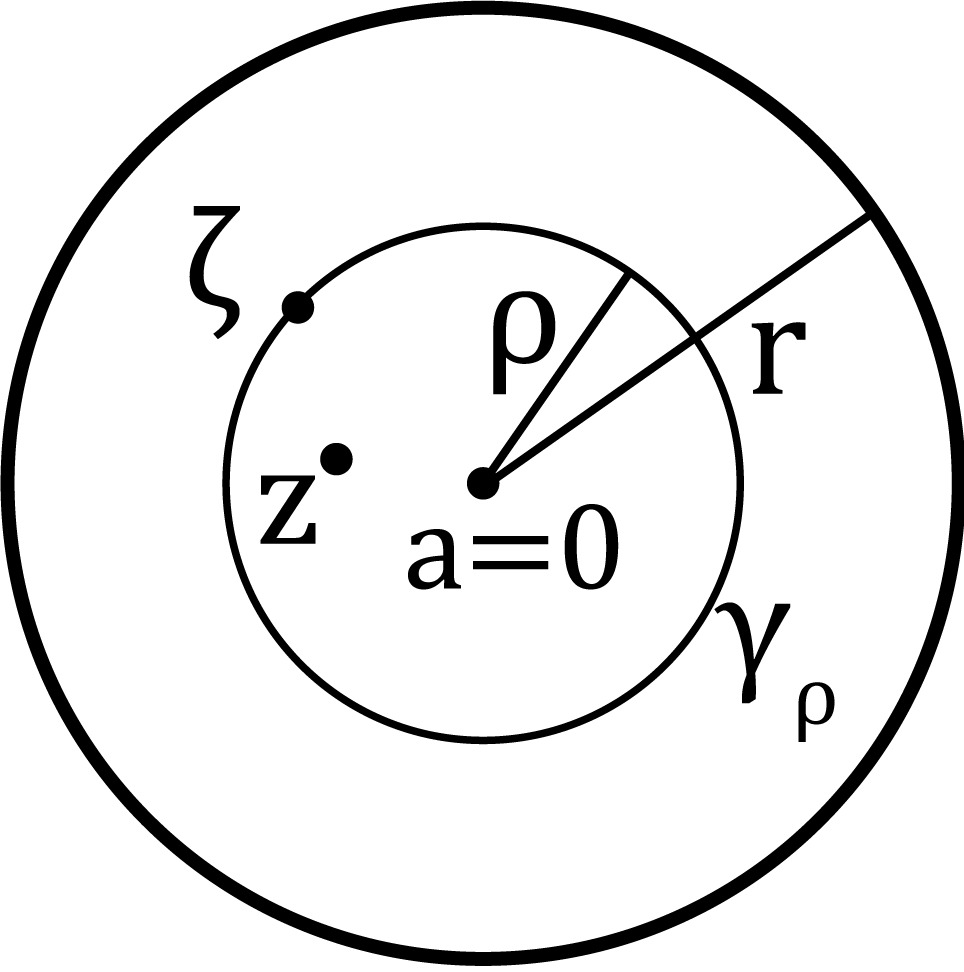
\includegraphics[width=4cm]{11_22}
        \end{figure}
        По инт. ф-ле Коши\\
        Для $z$ выберем $\rho$ : $\abs{z} < \rho < r$
        \[\gamma_\rho : \xi = a + \rho e^{it}\]
        \[f(z) = \frac{1}{2\pi i} \int_{\gamma_\rho} \frac{f(\xi)}{\xi - z} d\xi =
            \frac{1}{2\pi i}\int \frac{f(\xi)}{\xi(1 - \frac{z}{\xi})} d\xi \os{*}{=} \qq
        \abs{\frac{z}{\xi}} < 1\]
        \[\frac{1}{1 - \frac{z}{\xi}} = \sum_{ k =0}^\infty (\frac{z}{\xi})^k \q
        (\text{т.к. } \abs{\frac{z}{\xi}} < 1)\]
        \[\os{*}{=} \frac{1}{2\pi i} \int_{\gamma_\rho} f(\xi) \frac{1}{\xi}
        \sum_{k = 0}^\infty \frac{z^k}{\xi^k}d\xi = \frac{1}{2\pi i} \sum_{k = 0}^\infty
        z^k \int_{\gamma_\rho} \frac{f(\xi)}{\xi^{k + 1} }d\xi \]
        \begin{figure}[H]
          \centering
          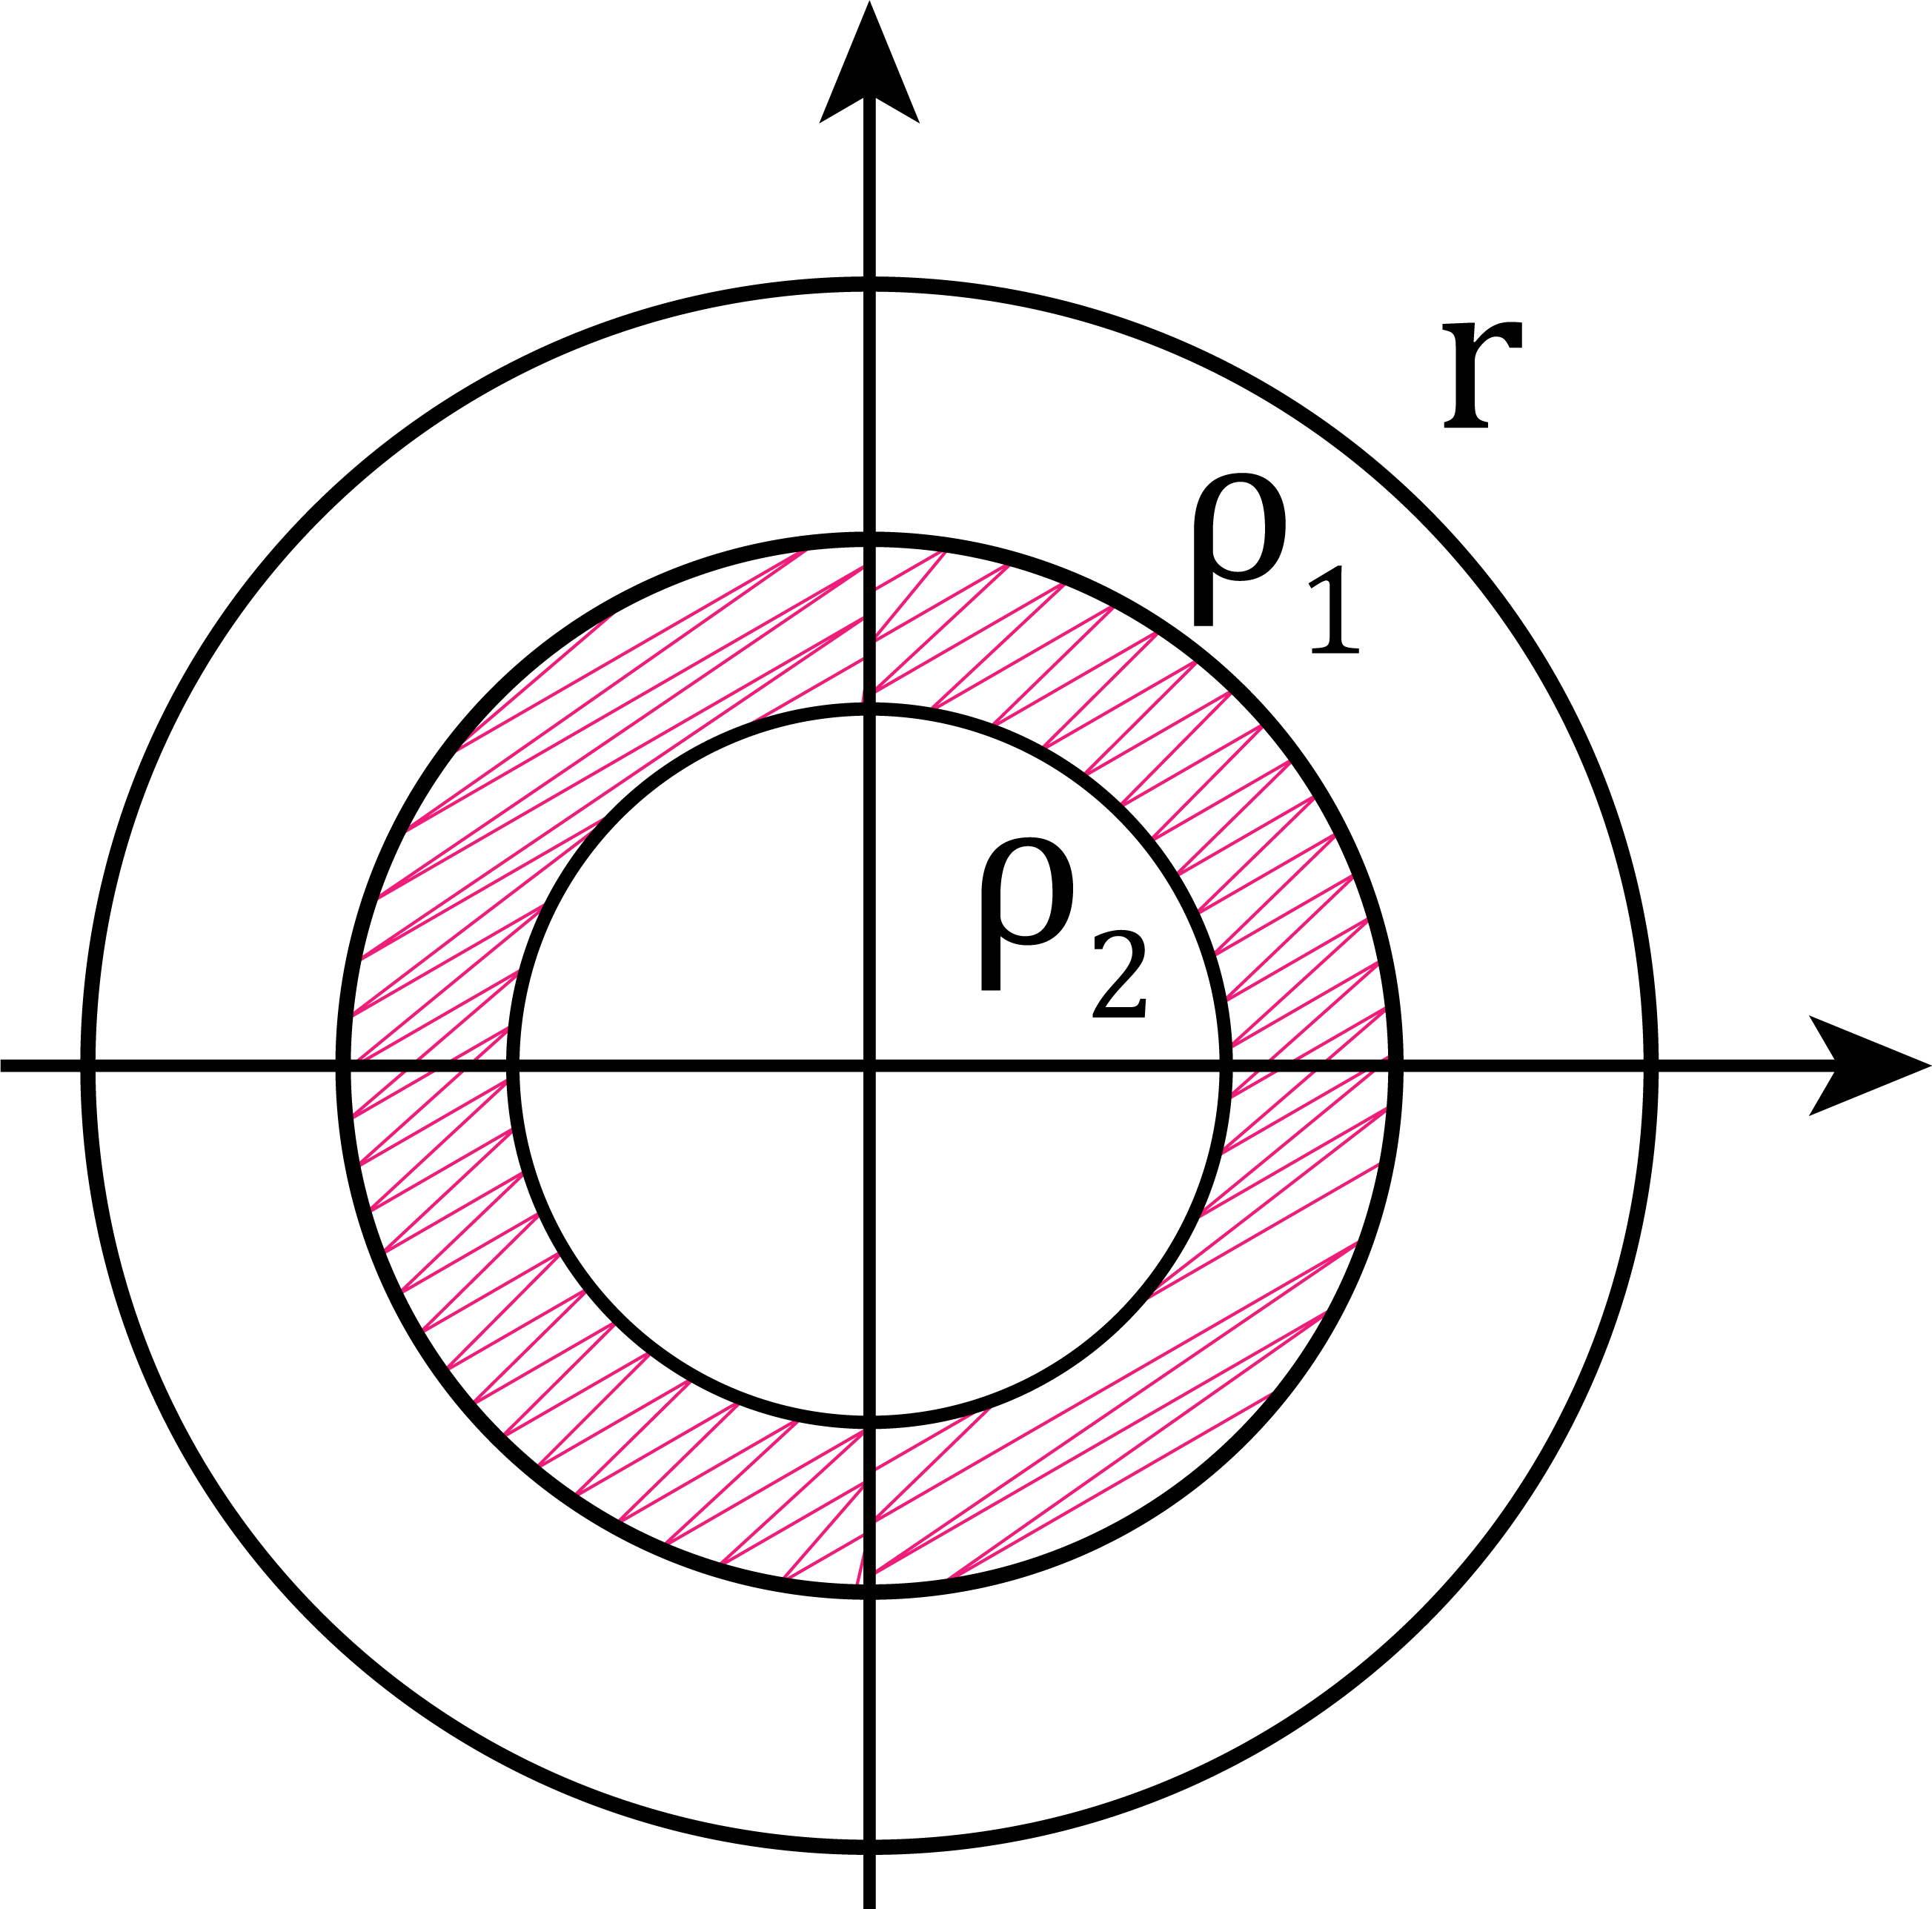
\includegraphics[width=5cm]{11_23}
        \end{figure}
        \[a_k = \frac{1}{2\pi i} \int_{\gamma_\rho} \frac{f(\xi) d\xi}{\xi^{k + 1} } =
        \frac{f^{(k)}(0) }{k!}\]
        \[\gamma_\rho \text{ - не зависит от } \rho\]
    \end{Proof}

    \begin{Definition} [инт. ф-ла Коши]
        \[f(z_0) = \frac{1}{2\pi i}\int_{\gamma_\rho} \frac{f(\xi)}{\xi - z_0} d\xi \]
    \end{Definition}

    \begin{Lemma}
        \[f^{(k)}(z_0) = \frac{k!}{2 \pi i} \int_{\gamma_\rho}
        \frac{f(\xi)}{(\xi - z_0)^{k + 1} }d\xi \]
    \end{Lemma}

    \begin{Consequence} [н-ва Коши]
        \[M(\rho) = \max_{\xi \in \gamma_\rho}  \abs{f(\xi)}\]
        \[f(z) = \sum_{k = 0}^\infty a_k \cdot z^k \qq (a = 0) \]
        \[\gamma_\rho : \q \abs{z} = \rho\]
        \[\abs{a_k} = \abs{\frac{1}{2\pi i} \int_{\gamma_\rho} \frac{f(\xi)d\xi}
        {\xi^{k + 1} } } \leq \frac{1}{2\pi} \cdot \frac{M(\rho)}{\rho^{k + 1}  \cdot 2 \pi
        \rho} = \frac{M(\rho)}{\rho^k}\]
        \[f \text{ - целая } \rla f \in H(\CC)\]
    \end{Consequence}

    \begin{Theorem} [Лиувилля]
        \[\text{Если } f \text{ - целая и огр } \Ra f(z) = const\]
    \end{Theorem}

    \begin{Proof}
        \[f \in H(\CC), \q \abs{f(z)} \leq M < \infty \qq \forall  z \in \CC\]
        \[\abs{a_k} \leq \frac{M}{\rho^k} \to 0 \q \rho \to  \infty \qq \forall k \neq 0\]
    \end{Proof}
\end{document}
